\chapter{Αστρικές ατμόσφαιρες}
\label{ch:Chapter4}

\section{Πεδία ακτινοβολίας και ιδιότητες}
Στα προηγούμενα κεφάλαια μιλήσαμε για ένταση και ροή ακτινοβολίας χωρίς να έχουμε ορίσει αυστηρά τι σημαίνουν αυτά τα μεγέθη. Σε αυτό το κεφάλαιο θα μιλήσουμε για τις ατμόσφαιρες των άστρων ξεκινώντας με το να δώσουμε επακριβείς ορισμούς συγκεκριμένων μεγεθών που χαρακτηρίζουν και περιγράφουν ένα πεδίο ακτινοβολίας.

\subsection{Η στερεά γωνία}
{\color{red} \hrule}
Στερεά γωνία είναι το κομμάτι της επιφάνειας που καλύπτει ένα αντικείμενο πάνω σε μία σφαίρα, όπως το βλέπει ένας παρατηρητής στο κέντρο της σφαίρας. Με άλλα λόγια, η στερεά γωνία δείχνει το οπτικό πεδίο που καταλαμβάνει το εν λόγω αντικείμενο από ένα συγκεκριμένο σημείο, είναι δηλαδή ένα μέτρο του πόσο μεγάλο φαίνεται το αντικείμενο στον παρατηρητή.\\
 {\color{red} \hrule}
Πριν ορίσουμε το τι είναι η στερεά γωνία, ας θυμηθούμε πως ορίζουμε τις επίπεδες γωνίες (plane angles) στις δύο διαστάσεις. Η γωνία ορίζεται ως ο λόγος του μήκους τόξου (arc length) που φαίνεται από αυτή τη γωνία προς την ακτίνα του κύκλου (σχήμα \ref{fig:plane_and_solid_angle}). 
\begin{equation}
\label{eq:plane_angle}
    \theta = \frac{l}{r}
\end{equation}

\begin{figure}[h]
   \centering
\begin{subfigure}[h]{0.45\textwidth}
	\centering
   	 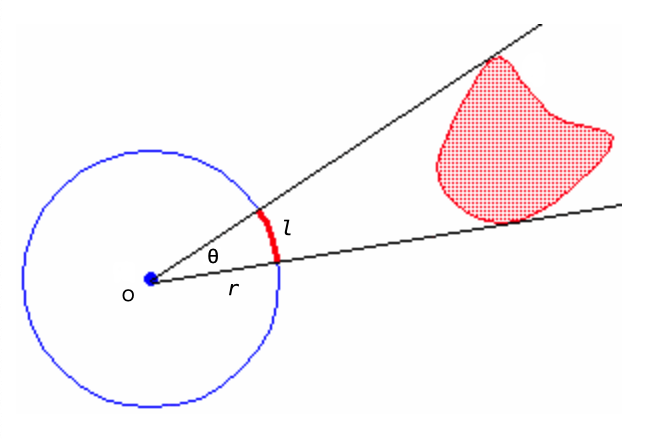
\includegraphics[scale=0.3]{Figures/plane_angle_def.png} 
\end{subfigure}
\begin{subfigure}[h]{0.5\textwidth}
	\centering
	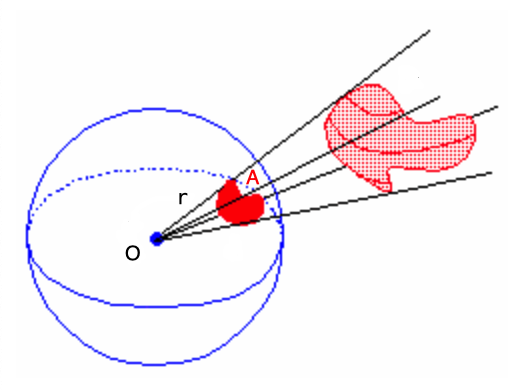
\includegraphics[scale=0.3]{Figures/solid_angle_def.png} 
    \end{subfigure}
    \caption{Ορισμός α) επίπεδης γωνίας και β) στερεάς γωνίας.}
    \label{fig:plane_and_solid_angle}
\end{figure}


Για τον μοναδιαίο κύκλο ($r=1$), ένας πλήρης κύκλος έχει $2\pi$ ακτίνια (rad). Κατα τα γνωστά, η επιφάνεια του κύκλου (ή πιο σωστά δίσκου) θα είναι $A = \pi r^2$ και η περιφέρειά του $C = 2 \pi r$.

Κατα αντιστοιχία, η στερεά γωνία είναι η μεταφορά της επίπεδης γωνίας στον τρισδιάστατο χώρο, και όπως η επίπεδη γωνία είναι και αυτή αδιάστατο μέγεθος. Ορίζεται ως ο λόγος της επιφάνειας που προβάλλεται πάνω σε μία σφαίρα προς το τετράγωνο της ακτίνας της σφαίρας (σχήμα \ref{fig:plane_and_solid_angle}).

\begin{equation}
    \label{eq:solid_angle}
    \Omega = \rm \frac{projected \ area}{distance ^2}=\frac{A}{r^2}
\end{equation}

Η αδιάστατη μονάδα με την οποία μετράμε τις στερεές γωνίες, ονομάζεται \textit{στερακτίνιο ή steradian (sr)}. Υποθέτοντας για απλότητα ότι η επιφάνεια $A$ είναι σφαίρα και γνωρίζοντας ότι η επιφάνεια σφαίρας δίνεται από τη σχέση $A = 4\pi r^2$, γίνεται αντιληπτό πως αν η επιφάνεια $A$ καλύπτει όλη τη σφαίρα, τότε $\Omega = 4 \pi$. Άρα μία σφαίρα έχει $4 \pi$ sr.\\


\begin{figure}[h]
    \centering
    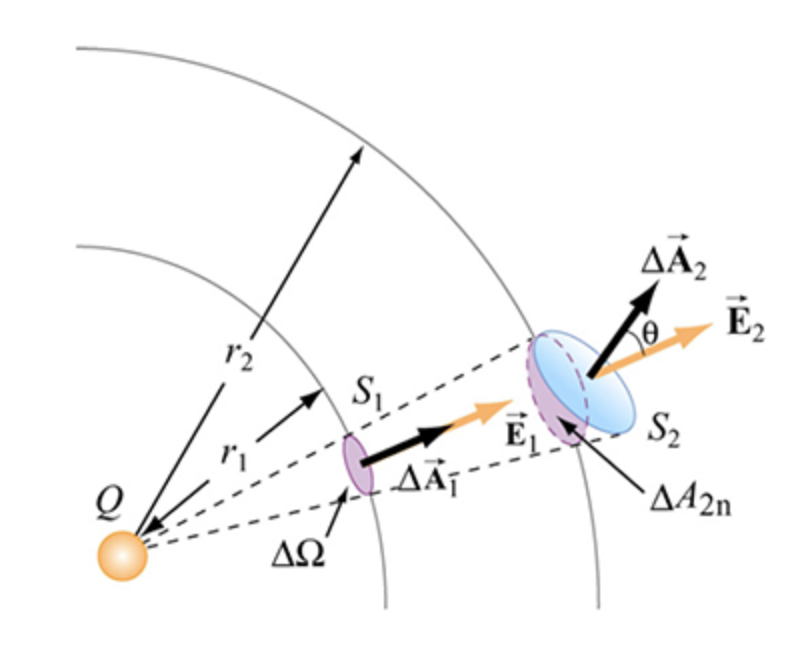
\includegraphics[scale=0.6]{Figures/solid_angle_projection.png}
    \caption{Υπολογισμός στερεάς γωνίας $\Delta \Omega$ μέσω της διανυσματικής επιφάνειας $S_2$.}
    \label{fig:solid_angle_projection}
\end{figure}

Στο σχήμα \ref{fig:solid_angle_projection} φαίνονται δύο διανυσματικές επιφάνειες $\boldsymbol{S}_1 = S_1 \Delta \boldsymbol{A}_1$ και $\boldsymbol{S}_2 = S_2 \Delta \boldsymbol{A}_2$, όπου $\Delta \boldsymbol{A}_1$ και $\Delta \boldsymbol{A}_2$ είναι τα διανύσματα κάθετα (normal) στις επιφάνειες $S_1$ και $S_2$, ενώ απέχουν αποστάσεις $r_1$ και $r_2$ αντίστοιχα από κέντρο σφαίρας Q.
Το διάνυσμα $\Delta \boldsymbol{A}_1$ είναι παράλληλο με το ακτινικό μοναδιαίο διάνυσμα $\boldsymbol{\hat{r}}$, όπου $\boldsymbol{\hat{r}} = \frac{\boldsymbol{r}}{r}$ και το οποίο έχει διεύθυνση τον άξονα του κώνου που σχηματίζει στερεά γωνία $\Delta \Omega$. Με άλλα λόγια, η επιφάνεια $S_1$ είναι κάθετη στο ακτινικό διάνυσμα $\boldsymbol{\hat{r}}$.

Έτσι, η στερεά γωνία υπολογισμένη για την επιφάνεια $S_1$ θα είναι:
$$\Delta \Omega = \frac{\boldsymbol{S}_1 \cdot \boldsymbol{\hat{r}}}{r_1^2} = \frac{S_1 \cancelto{1}{|\boldsymbol{\hat{r}}|} \cancelto{1}{\cos(\Delta \boldsymbol{A}_1, \boldsymbol{\hat{r}})}}{r_1^2} = \frac{S_1}{r_1^2}$$

Το διάνυσμα $\Delta \boldsymbol{A}_2$ βρίσκεται υπο γωνία $\theta$ σε σχέση με το ακτινικό μοναδιαίο διάνυσμα $\boldsymbol{\hat{r}}$. Γι' αυτό το λόγο, πρέπει να προβάλουμε την επιφάνεια $\Delta \boldsymbol{A}_2$ σε μια επιφάνεια $\Delta \boldsymbol{A}_{2n}$ η οποία θα έχει κατεύθυνση ίδια με αυτή του $\boldsymbol{\hat{r}}$. Η προβολή θα είναι: $$\Delta \boldsymbol{A}_{2n} = \rm proj_{\boldsymbol{\hat{r}}} \boldsymbol{S}_2 = \frac{\boldsymbol{S}_2 \cdot \boldsymbol{\hat{r}}}{|\boldsymbol{\hat{r}}|^2}\boldsymbol{\hat{r}} = \frac{S_2 \cancelto{1}{|\boldsymbol{\hat{r}}|} \cos (\Delta \boldsymbol{A}_2, \boldsymbol{\hat{r}})}{\cancelto{1}{|\boldsymbol{\hat{r}}|^2}}\boldsymbol{\hat{r}} = S_2 \cos \theta \ \boldsymbol{\hat{r}}$$

Άρα, η στερεά γωνία υπολογισμένη για την επιφάνεια $S_2$ θα είναι:
$$\Delta \Omega = \frac{\Delta \boldsymbol{A}_{2n} \cdot \boldsymbol{\hat{r}}}{r_2^2} = \frac{S_2 \cos \theta \cancelto{1}{|\boldsymbol{\hat{r}}|} \cancelto{1}{\cos (\boldsymbol{\hat{r}}, \boldsymbol{\hat{r}})}}{r_2^2} = \frac{S_2 \cos \theta}{r_2^2}$$



Είναι χρήσιμο όταν θέλουμε να υπολογίσουμε ολοκληρώματα στερεών γωνιών να τα μετατρέψουμε σε σφαιρικές συντεταγμένες. Από το σχήμα \ref{fig:diff_solid_angle} προκύπτει ότι η γωνία $d \theta$ βάσει του ορισμού της επίπεδης γωνίας (σχέση \eqref{eq:plane_angle}) θα είναι $d \theta = \frac{s_{\theta}}{r}$ όπου $s_{\theta}$ είναι το μήκος του τόξου (μπλε γραμμή στο σχήμα) που βλεπει τη γωνία $d \theta$. Αντίστοιχα, για την αζιμούθια γωνία\footnote{Δες και Παράρτημα \ref{apx:coordinates} αναφορικά με τις σφαιρικές συντεταγμένες.} $d \phi = \frac{s_{\phi}}{r \sin \theta}$. Συνεπώς η διαφορική επιφάνεια $dA$ είναι:
$$dA = s_{\theta} \times s_{\phi} = r d\theta \times r \sin \theta d \phi = r^2 \sin \theta d \phi d \theta$$
και άρα 
\begin{equation}
    \label{eq:diff_solid_angle}
    d \omega = \frac{dA}{r^2} = \sin \theta d \theta d \phi
\end{equation}
Η στερεά γωνία τότε είναι
\begin{equation}
    \label{eq:solid_angle_integral}
    \Omega = \iint_S d \omega = \int_{\phi_1}^{\phi_2} \int_{\theta_1}^{\theta_2} \sin \theta d \theta d \phi = (\phi_2 - \phi_1)(\cos \theta_1 - \cos \theta_2)
\end{equation}


\begin{figure}[h]
    \centering
    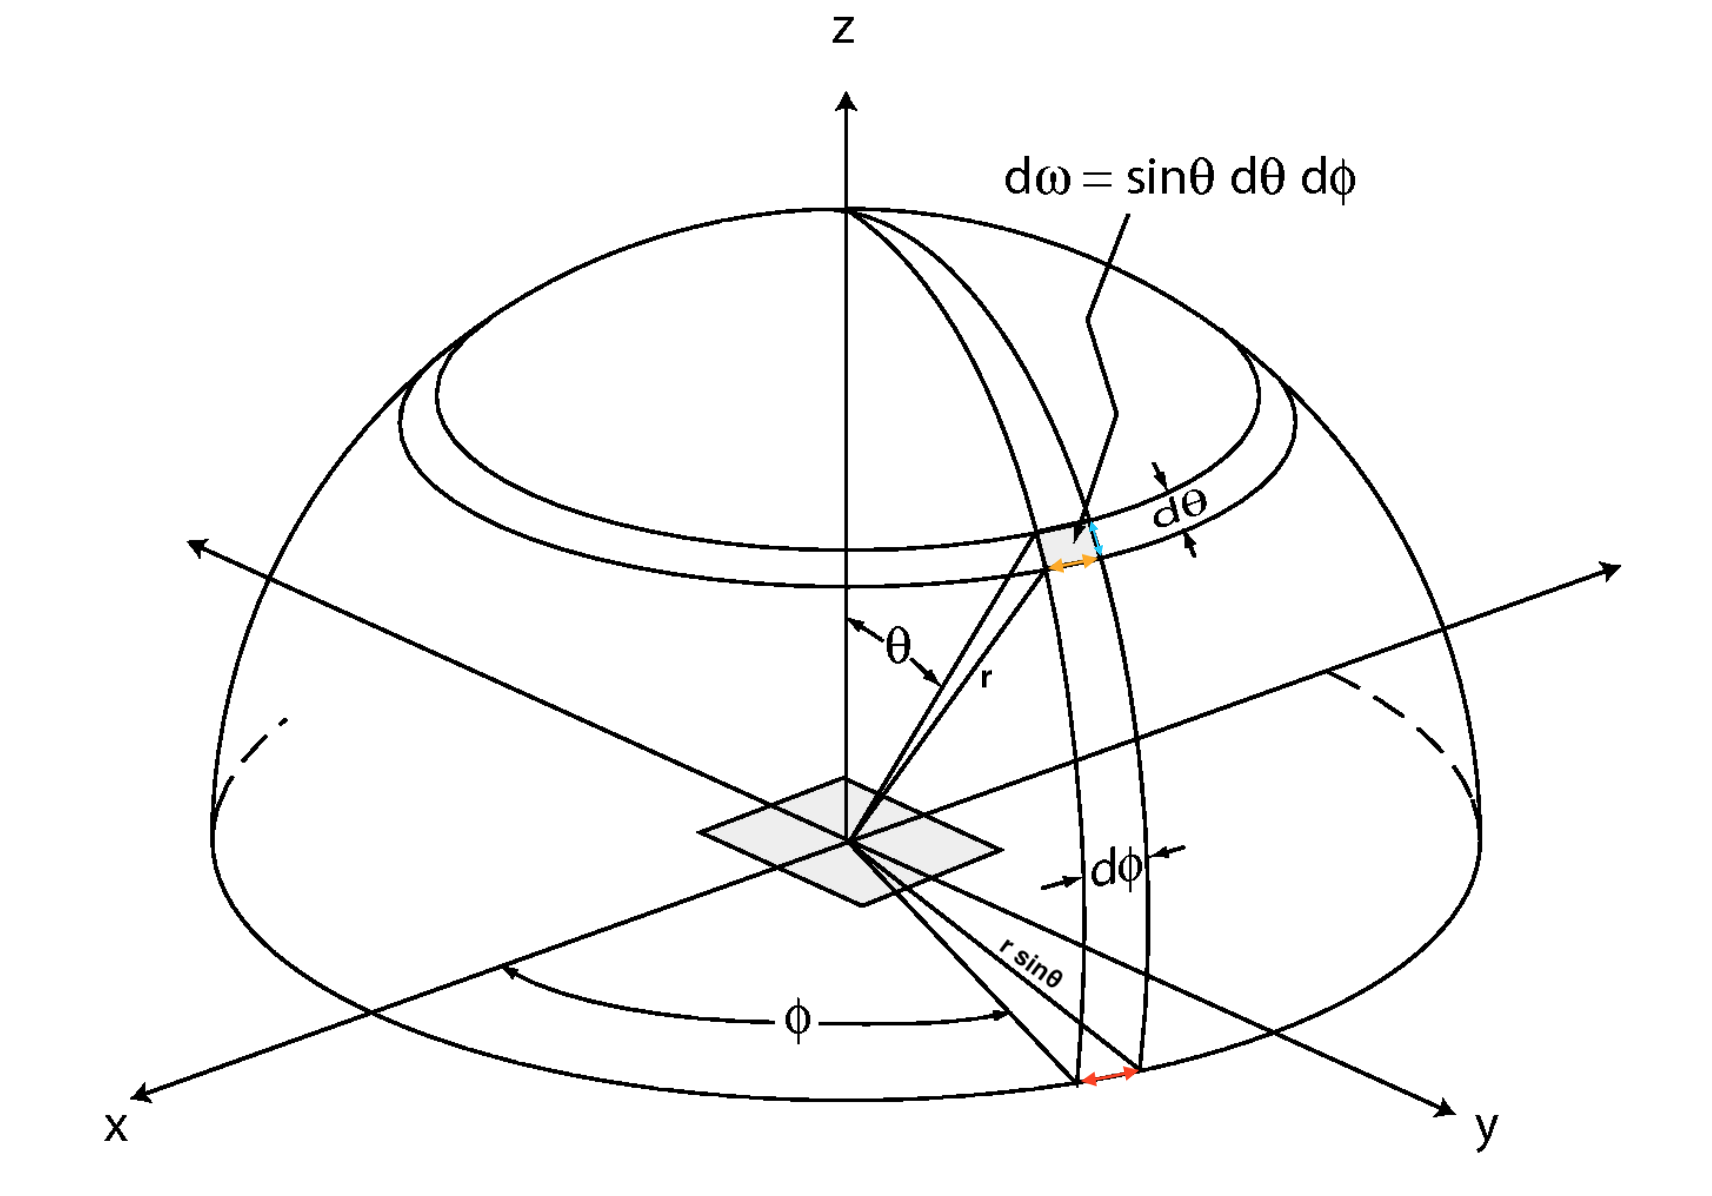
\includegraphics[scale=0.3]{Figures/diferential_solid_angle.png}
    \caption{Διαφορική στερεά γωνία σε σφαιρικές συντεταγμένες.}
    \label{fig:diff_solid_angle}
\end{figure}

\textbf{Έχοντας ως δεδομένα πως η μέση απόσταση Γης-Σελήνης και Γης-Ήλιου είναι $D_{EM} = 3.84 \times 10^5 \ \rm km$ και $D_{ES} = 1.496 \times 10^8 \ \rm km$ αντίστοιχα, και επιπρόσθετα $R_M = 1.74 \times 10^3 \ \rm km$, $R_S = 6.96 \times 10^5 \ \rm km$ είναι η ακτίνα της Σελήνης και του Ήλιου αντίστοιχα, να βρείτε: α) Ποιά είναι η γωνιακή διάμετρος του Ήλιου και της Σελήνης, β) Ποιά είναι η στερεά γωνία υπό την οποία φαίνονται ο Ήλιος και η Σελήνη από τη Γη, και γ) Ποιό από τα δύο αντικείμενα εμφανίζεται μεγαλύτερο;}

\begin{figure}[h]
    \centering
    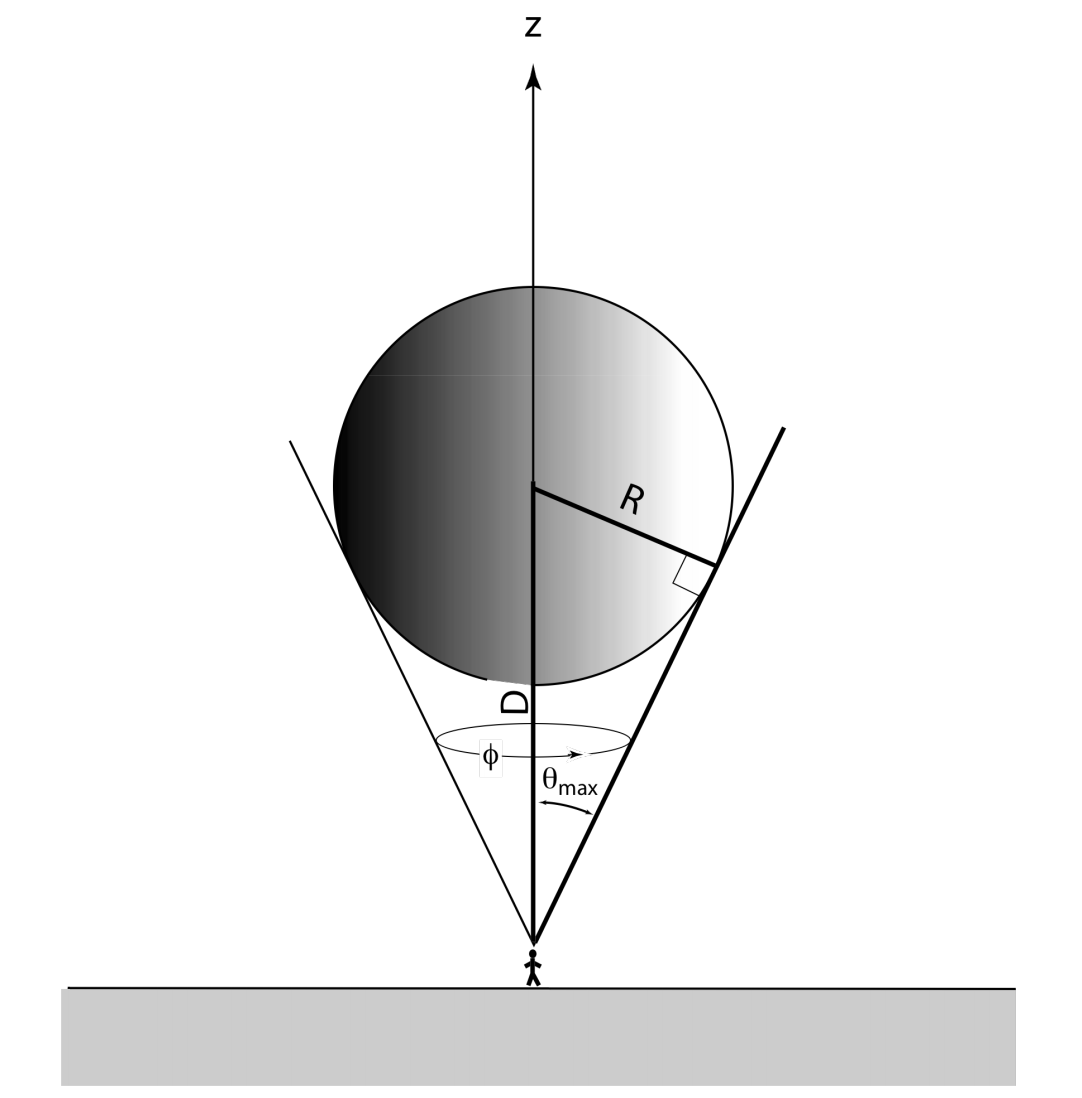
\includegraphics[scale=0.5]{Figures/solid_angle_problem.png}
    \caption{Γεωμετρικό πλαίσιο για τον υπολογισμό της στερεάς γωνίας υπό την οποία φαίνεται σφαίρα ακτίνας R της οποιάς το κέντρο βρίσκεται σε απόσταση D από τον παρατηρητή.}
    \label{fig:solid_angle_problem}
\end{figure}

Για το πρώτο ερώτημα, χρησιμοποιώντας της σχέση \eqref{eq:angular_diameter} και από το σχήμα \ref{fig:solid_angle_problem} μπορούμε να γράψουμε:
$$\theta_{\rm max} = \arcsin \left( \frac{R}{D} \right)$$ από την οποία προκύπτει $2\theta_{\rm max}^{M} = 0.52^{\circ}$ για τη Σελήνη και $2\theta_{\rm max}^{S} = 0.53^{\circ}$.

Για το δεύτερο ερώτημα, η στερεά γωνία με άνοιγμα $2\theta$ θα είναι βάσει της σχέσης \eqref{eq:diff_solid_angle}:
$$\Omega = \int_{0}^{2\pi} \int_{0}^{\theta} \sin \theta d \theta d \phi = 2\pi (1 - \cos \theta)$$ από την οποία προκύπτει $\Omega_M = 6.5 \times 10^{-5} \ \rm sr$ για τη Σελήνη και $\Omega_S = 6.8 \times 10^{-5} \ \rm sr$ για τον Ήλιο.

Για το τρίτο ερώτημα, προκύπτει ότι ο Ήλιος καταλαμβάνει 5\% μεγαλύτερη στερεά γωνία από τη Σελήνη. Το γεγονός ότι χρησιμοποίησαμε τις μέσες αποστάσεις Γης-Σελήνης και Ήλιου-Σελήνης για τους παραπανω υπολογισμούς και ότι γενικά αυτές οι τιμές δεν είναι σταθερές, εξηγεί την ύπαρξη ολικών εκλείψεων Ηλίου.
{\hrule}



\subsection{Η έννοια της έντασης ακτινοβολίας}
Όπως έχουμε πει, ο ρυθμός με τον οποίο τα αστέρια ακτινοβολούν ενέργεια ονομάζεται \textit{λαμπρότητα} (luminosity) και μετριέται σε J/s (Watt) ή erg/s. Η λαμπρότητα είναι μία ενδογενής ιδιότητα του αστέρα. 

Τι συμβαίνει όμως στο φως που ακτινοβολείται από τα αστέρια όσο αυτό κινείται προς το μέρος μας; Οι ακτίνες φωτός ``ανοίγουν" με την απόσταση που σημαίνει ότι λιγότερο φως περνάει από έναν ανιχνευτή μιας συγκεκριμένης διατομής όσο μεγαλώνει η απόσταση. Με άλλα λόγια, ο αστέρας εμφανίζεται αμυδρότερος. Έτσι, ορίζουμε την ενέργεια που περνάει \textit{\color{red} ανεξαρτήτως διεύθυνσης} από μια επιφάνεια $\rm 1 m^2$ ανα δευτερόλεπτο ως \textit{ροή} (flux, irradiance ή radiosity). Η ροή μετριέται σε W/$\rm m^2$ ή $\rm ergs \ s^{-1} \ cm^{-2}$. 



\subsubsection{Ορισμός ειδικής έντασης ακτινοβολίας}
Η ροή ως μέγεθος δεν μας δίνει πολλές πληροφορίες καθώς δεν μας λέει από ποιά διεύθυνση προέρχεται το φως. Γι' αυτό ορίζουμε ένα νέο μέγεθος, την \textit{ειδική ένταση} ακτινοβολίας (specific intensity, spectral radiance ή spectral brightness) η οποία ορίζεται ως η ροή των φωτονίων συχνότητας $d \nu$ που διέρχονται \textit{\color{red} κάθετα} από σημείο, Ο, μιας επιφάνειας $dA_{\perp}$ και που εμπεριέχονται σε κάποια στερεά γωνία $d \omega$ της οποίας η διεύθυνση είναι $\boldsymbol{\hat{\Omega}}$. Από τον ορισμό της, η ειδική ένταση μετριέται σε $\rm W \ m^{-2} \ sr^{-1} \ Hz^{-1}$ ή $\rm ergs \ s^{-1} \ cm^{-2} \ sr^{-1} \ Hz^{-1}$ και δίνεται από τη σχέση:
\begin{equation}
    I_{\nu}(O, \boldsymbol{\hat{\Omega}}) = \frac{dE}{dt d\nu d\omega dA_{\perp}} = \frac{dP}{d\nu d\omega dA_{\perp}}
\end{equation}

Η ειδική ένταση της ακτινοβολίας χαρακτηρίζει σχεδόν πλήρως το πεδίο της ακτινοβολίας αφού η μόνο πληροφορία που δεν εμπεριέχεται είναι αυτή της πόλωσης του φωτός. Αν εξαιρέσουμε την πόλωση, η ειδική ένταση μας δείχνει πόσα φωτόνια και με τι ενέργειες είναι παρόντα καθώς και σε ποιά συγκεκριμένη διεύθυνση κινούνται. Όλες οι άλλες ποσότητες (π.χ. η ροή μέσω κάποιας συγκεκριμένης επιφάνειας προσανατολισμένης προς κάποια συγκεκριμένη διεύθυνση, η πίεση της ακτινοβολίας, η πυκνότητα ενέργειας κτλ) μπορούν να βρεθούν μέσω της έντασης (για λόγους συντομίας θα χρησιμοποιείται ο όρος ``ένταση" για να εκφράσουμε την ειδική ένταση. Όταν αναφερόμαστε στην ένταση όλων των συχνοτήτων θα γίνεται χρήση του όρου ``ολική ένταση").

Αν η επιφάνεια από την οποία διέρχονται τα φωτόνια βρίσκεται υπό γωνία, τότε η ροή υπολογίζεται βάσει της προβολής της επιφάνειας στο επίπεδο που βρίσκεται κάθετα στη διεύθυνση των ακτίνων ενώ ισχύει $$dA_{\perp} = dA \cos \theta \leq dA$$ όπου $\theta$ είναι γωνία που σχηματίζεται μεταξύ του κάθετος διανύσματος, $\boldsymbol{\hat{\eta}}$, στην επιφάνεια $dA$ και την κάθετη (στην πορεία των φωτονίων) επιφάνεια $dA_{\perp}$ με κατεύθυνση αυτή του διανύσματος $\boldsymbol{\hat{\Omega}}$ (νόμος συνημιτόνων Lambert, σχήμα \ref{fig:intensity_definition}). Άρα, η ειδική ένταση της ακτινοβολίας γράφεται γενικά:
\begin{equation}
    \label{eq:specific_intensity_def}
    I_{\nu}(O, \theta, \phi) = \frac{dE}{dt d\nu d\omega dA_{\perp}} = \frac{dP}{d\nu d\omega dA \cos \theta} \longrightarrow I_{\nu}(\theta) = I_{\nu}(0)\cos \theta
\end{equation}
όπου πλέον η επιφάνεια $dA$ είναι μία τυχαία επιφάνεια που σχηματίζει γωνία $\theta$ με την κάθετη επιφάνεια κατά τη διεύθυνση της ακτινοβολίας, $dA_{\perp}$. Η διεύθυνση δίνεται από τις γωνίες $\theta$ (πολική) και $\phi$ (αζιμούθια).

\begin{figure}[h]
   \centering
\begin{subfigure}[h]{0.45\textwidth}
	\centering
   	 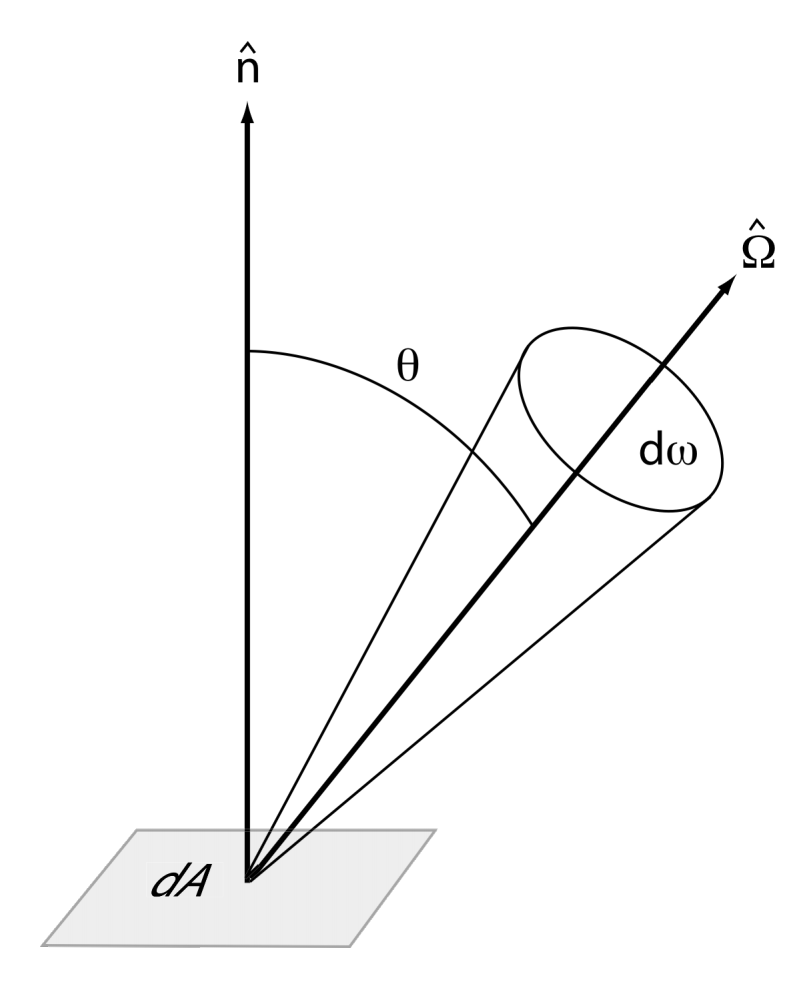
\includegraphics[scale=0.4]{Figures/specific_intensity_def_3D.png} 
\end{subfigure}
\begin{subfigure}[h]{0.5\textwidth}
	\centering
	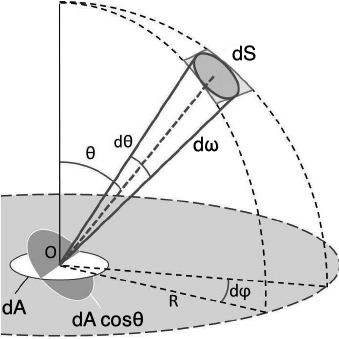
\includegraphics[scale=0.5]{Figures/specific_intensity_example.png} 
    \end{subfigure}
    \caption{Ορισμός της ειδικής έντασης ακτινοβολίας. Η συνεισφορά της ροής φωτονίων υπο γωνία $\theta$ πρέπει να ``ζυγιστεί'' με το συνημίτονο της γωνίας καθώς ισχύει $\cos \theta = \boldsymbol{\hat{\eta}} \cdot \boldsymbol{\hat{\Omega}}$. Η προβαλλόμενη επίπεδη επιφάνεια $dA_{\perp}$ είναι κάθετη στην διεύθυνση $(\theta_r, \phi_r)$, ενώ η επιφάνεια $dS$ που ``βλέπει'' το σημείο Ο ορίζει τη στερεά γωνία $d \omega = dS/R^2$, όπου $R$ η ακτίνα της σφαίρας με κέντρο το σημείο Ο.}
    \label{fig:intensity_definition}
\end{figure}

Το ότι μια τυχαία επιφάνεια $dA$ καταλαμβάνει μεγαλύτερη έκταση από την κάθετη επιφάνεια στη διεύθυνση διάδοσης της ακτινοβολίας φαίνεται καλύτερα στο σχήμα \ref{fig:oblique_rays}. Επειδή η ένταση της ακτινοβολίας δεν εξαρτάται από την απόσταση, το ίδιο ποσό ενέργειας μοιράζεται σε μεγαλύτερη επιφάνεια στην περίπτωση που αυτή δεν είναι κάθετη στην διεύθυνση διάδοσης της δέσμης.

\begin{figure}[h]
    \centering
    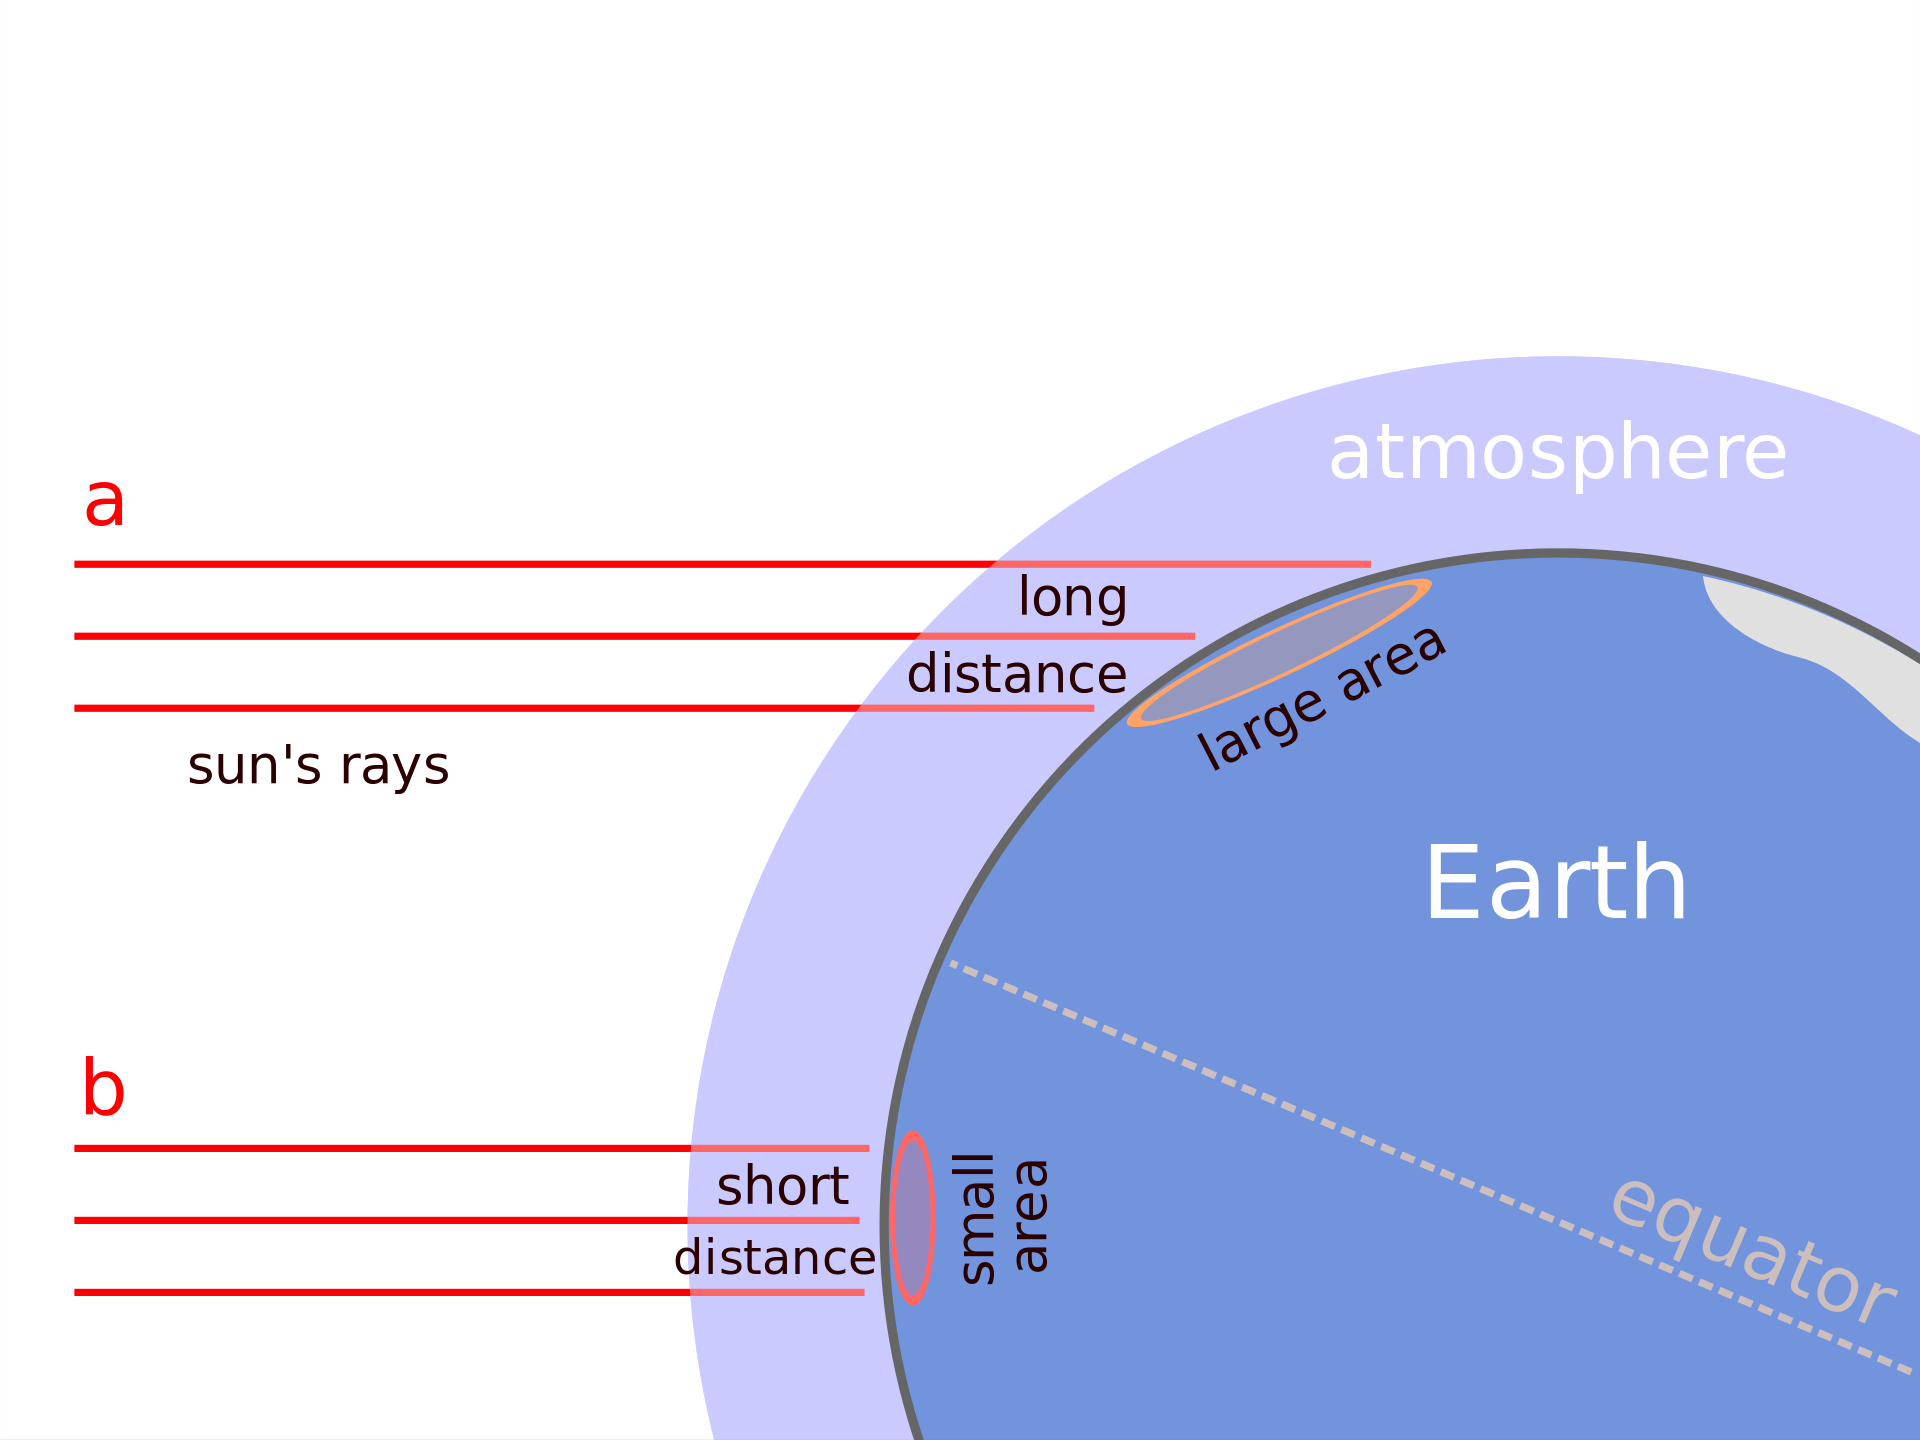
\includegraphics[scale=0.15]{Figures/oblique_rays.png}
    \caption{Γραφική απεικόνιση της εξάρτησης της έντασης ακτινοβολίας από τη γωνία που σχηματίζει η επιφάνεια με τη διεύθυνση διάδοσης της ακτινοβολίας.}
    \label{fig:oblique_rays}
\end{figure}



\subsubsection{Ιδιότητες της ειδικής έντασης ακτινοβολίας}
Η ένταση της ακτινοβολίας παραμένει αναλλοίωτη (σταθερή) κατά τη διεύθυνση της δέσμης με την προϋπόθεση ότι δεν παρεμβάλλονται άλλες πηγές ή καταβόθρες μεταξύ της πηγής και του δέκτη. Αυτό αποδεικνύεται γεωμετρικά ως εξής: θεωρούμε δύο επιφάνειες $dA$ και $dS$ όπου η μία εκπέμπει φως ενω ή άλλη λειτουργεί ως δέκτης (σχήμα \ref{fig:intensity_invariance}).

\begin{figure}[h]
    \centering
    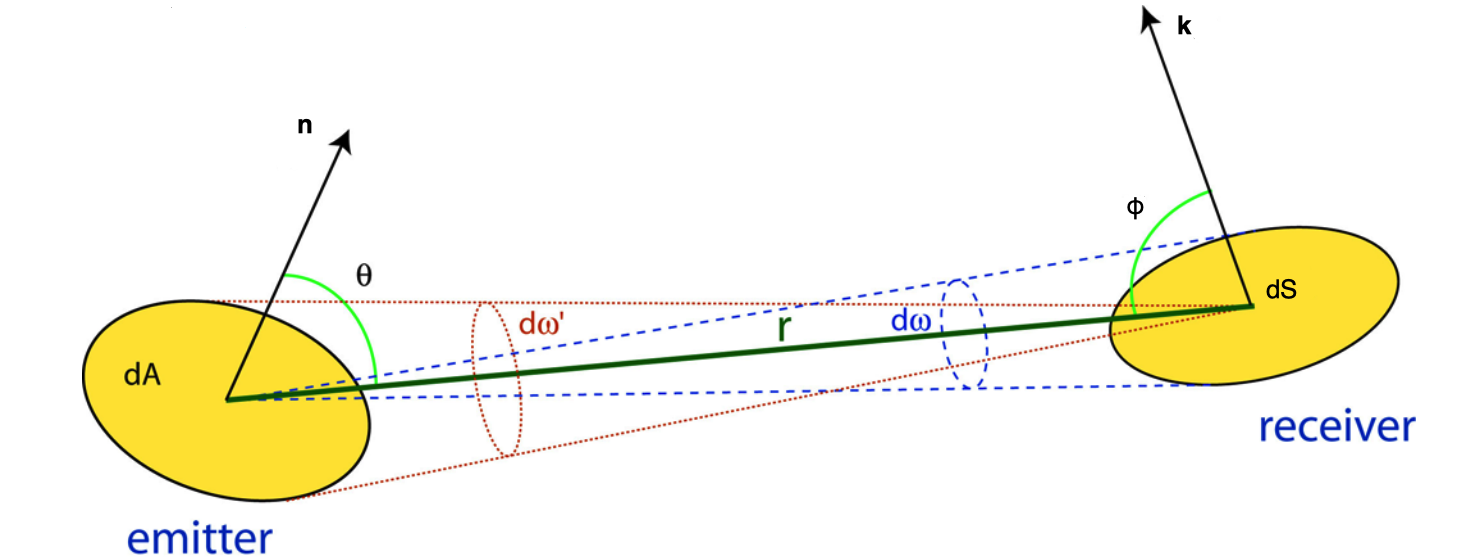
\includegraphics[width=\linewidth]{Figures/intensity_invariance.png}
    \caption{Γεωμετρική αναπαράσταση της διατήρησης της έντασης ακτινοβολίας κατα μήκος μιας ακτίνας φωτός.}
    \label{fig:intensity_invariance}
\end{figure}

Έστω ότι $d\omega$ είναι η στερεά γωνία που σχηματίζει η επιφάνεια του δέκτη $dS$, όπως φαίνεται από το κέντρο της επιφάνειας $dA$ (πηγή).

Αντίστοιχα, έστω ότι $d \omega^{\prime}$ είναι η στερεά γωνία που σχηματίζει η επιφάνεια της πηγής $dA$, όπως φαίνεται από το κέντρο της επιφάνειας $dS$ (δέκτης). Τότε, σύμφωνα με τον ορισμό της στερεάς γωνίας (σχέση \eqref{eq:solid_angle}) θα έχουμε:

\begin{eqnarray*}
    d\omega = \frac{dS \cos \phi}{r^2} \\ \\
    d\omega^{\prime} = \frac{dA \cos \theta}{r^2}
\end{eqnarray*}

Η ενέργεια που διέρχεται μέσα από την επιφάνεια $dA$ με στερεά γωνία $d\omega$ σύμφωνα με τη σχέησ \eqref{eq:specific_intensity_def} είναι:
\begin{equation*}
    dE = I_{\nu} dt d\nu d\omega dA \cos \theta = I_{\nu} dt d\nu \left( \frac{dS \cos \phi}{r^2} \right) dA \cos \theta
\end{equation*}

Αντίστοιχα, η ενέργεια που διέρχεται μέσα από την επιφάνεια του δέκτη $dS$ με στερεά γωνία $d\omega^{\prime}$ είναι:
\begin{equation*}
    dE^{\prime} = I_{\nu}^{\prime} dt d\nu d\omega^{\prime} dS \cos \phi = I_{\nu}^{\prime} dt d\nu \left( \frac{dA \cos \theta}{r^2} \right) dS \cos \phi
\end{equation*}

Εφόσον η ενέργεια που εκπέμπφθηκε από την πηγή δεν απορροφήθηκε από πουθενά θα ισχύει $$dE = dE^{\prime} \longrightarrow I_{\nu} = I_{\nu}^{\prime}$$

Το παραπάνω αποτέλεσμα έχει δύο πολύ σημαντικές ιδιότητες
\begin{itemize}
    \item Η ένταση της ακτινοβολίας είναι ανεξάρτητη της απόστασης.
    \item Η ένταση της ακτινοβολίας είναι ίδια και στην πηγή και στον δέκτη. Άρα μπορούμε να σκεφτούμε την ένταση με όρους ενέργειας που πηγάζει από κάπου ή ως ενέργεια που διέρχεται μέσα από έναν ανιχνευτή.
\end{itemize}

Η ολική ένταση 
\begin{equation}
    I \equiv \int_{0}^{\infty} I_{\nu} d\nu = \int_{0}^{\infty} I_{\lambda} d\lambda
\end{equation}
διατηρείται επίσης, ενώ ισχύει κατά τα γνωστά ότι $|I_{\nu} d\nu| = |I_{\lambda} d\lambda|$.




\subsection{Πυκνότητα ροής, μέση ένταση, πυκνότητα και πίεση ακτινοβολίας}

\subsubsection{Πυκνότητα ροής}
Εαν η πηγή είναι διακριτή, δηλαδή καταλαμβάνει μία καλώς ορισμένη στερεά γωνία, τότε η ``πυκνότητα ροής'', $S_{\nu}$,  είναι η ισχύς που λαμβάνει ένας ανιχνευτής ανα μονάδα προβαλλόμενης επιφάνειας και ανα συχνότητα. 
Απο τη σχέση \eqref{eq:specific_intensity_def} προκύπτει ότι
\begin{equation*}
    \frac{dP}{d\nu dA} = I_{\nu} \cos \theta d\omega
\end{equation*}
και ολοκληρώνοντας ώστε να πάρουμε την ενέργεια ανα μονάδα χρόνου και ανα συχνότητα που διαπερνάει μία οποιαδήποτε επιφάνεια ανεξάρτητα της κατεύθυνσης καταλήγουμε:

\begin{equation}
    \label{eq:flux_density_def}
    S_{\nu} = \int I_{\nu}(\theta, \phi) \cos \theta d\omega
\end{equation}

Αν το γωνιακό μέγεθος της πηγής είναι $\ll 1 \ \rm rad$ τότε $\cos \theta \approx 1$ και η σχέση \eqref{eq:flux_density_def} απλοποιείται στην:
\begin{equation}
    \label{eq:flux_density_simple}
    S_{\nu} = \int I_{\nu}(\theta, \phi) d\omega
\end{equation}
κάτι το οποίο ισχύει σχεδόν πάντα καθώς δεν είθισται να χρησιμοποιούμε την πυκνότητα ροής για μεγάλους στόχους στους οποίους θα χρειαζόταν να κρατήσουμε τον όρο του συνημιτόνου (π.χ. εκπομπή από τον Γαλαξία).\\

{\color{red} \hrule}
\textbf{Πότε όμως χρησιμοποιούμε την ειδική ένταση και πότε την πυκνότητα ροής για να περιγράψουμε μία πηγή};

Εάν η πηγή έχει πολύ μικρό γωνιακό μέγεθος ώστε να μπορεί να θεωρηθεί σημειακή, η πυκνότητα ροής μπορεί να μετρηθεί αλλά όχι η ειδική ένταση.
Εάν η πηγή έχει πολύ μεγάλο γωνιακό μέγεθος, τότε η ειδική ένταση μπορεί να μετρηθεί απευθείας σε κάθε σημείο της πηγής, αλλά η πυκνότητα ροής πρέπει να υπολογισθεί ολοκληρώνοντας την παρατηρήσιμη ένταση σε όλη τη στερεά γωνία που καταλαμβάνει η πηγή. Έτσι, η πυκνότητα ροής χρησιμοποιείται μόνο για να περιγράψει σχετικά μικρές πηγές.
{\color{red} \hrule}

Η πυκνότητα ροής μετριέται σε $\rm W \ m^{-2} \ Hz^{-1}$ ή $\rm ergs \ s^{-1} \ m^{-2} \ Hz^{-1}$. Επειδή όμως αυτές οι μονάδες είναι πολύ μεγάλες για τις τιμές που τυπικά μετράμε από αστρονομικά αντικείμενα, έχει υιοθετηθεί μία άλλη μονάδα, το Jansky (Jy) 
$$\rm 1 \ Jy \equiv 10^{-26} W \ m^{-2} \ Hz^{-1} \equiv 10^{-23} ergs \ s^{-1} \ m^{-2} \ Hz^{-1}$$

Σε αντίθεση με την ένταση της ακτινονολίας, η πυκνότητα ροής δεν είναι ανεξάρτητη της απόστασης. Επειδή $$\int d\omega \propto d^{-2} \longrightarrow S_{\nu} \propto d^{-2}$$ το οποίο είναι γνωστό ως νόμος του αντίστροφου τετραγώνου. Άρα κάποια αστέρια φαίνονται αμυδρά επειδή καταλαμβάνουν μικρότερη στερεά γωνία στον ουράνιο θόλο (και άρα έχουν μικρότερη ροή) και όχι επειδή η ένταση της ακτινοβολίας μειώνεται με την απόσταση.

Ολοκληρώνοντας σε όλες τις συχνότητες, παίρνουμε την γνωστή (ολική) ροή (ισχύς ανά μονάδα επιφάνειας) ακτινοβολίας, αν και πολλές φορές ο όρος ``ροή'' χρησιμοποιείται έναντι του όρου ``πυκνότητα ροής'' για λόγους συντομίας:
\begin{equation}
    F_{\rm rad} \equiv S = \int_{0}^{\infty} S_{\nu} d\nu
\end{equation}

Τέλος, η λαμπρότητα σε ένα εύρος συχνοτήτων ορίζεται ως ισχύς ανά συχνότητα
(για πηγή που εκπέμπει ισοτροπικά):
\begin{equation}
    L_{\nu} = 4\pi d^2 S_{\nu} \longrightarrow L \equiv \int_{0}^{\infty} L_{\nu} d\nu
\end{equation}
και είναι ενδογενής ιδιότητα της πηγής καθώς δεν εξαρτάται από την απόσταση.



\subsubsection{Μέση ένταση ακτινοβολίας}
Η μέση ένταση της ακτινοβολίας είναι η \textit{ροπή μηδενικής τάξης της έντασης ως προς την ποσότητα $\cos \theta$}. Με άλλα λόγια, είναι η μέση τιμή της έντασης σε όλες τις στερεές γωνίες. Έτσι, έχουμε:
\begin{eqnarray*}
    J_{\nu} &=& \frac{\oint I_{\nu} d\omega}{\oint d\omega}, \ \rm \ με \ \ \oint d\omega = \int_{0}^{2\pi} \int_{0}^{\pi} \sin \theta d\theta d\phi = 4\pi \\ \\
    J_{\nu} &=& \frac{1}{4\pi} \int_{0}^{2\pi} \int_{0}^{\pi} I_{\nu}(\theta, \phi) \sin \theta d\theta d\phi
\end{eqnarray*}
Αν υποθέσουμε και αζιμουθαϊκή συμμετρία, τότε η παραπάνω σχέση γράφεται:
\begin{equation*}
    J_{\nu} = \frac{1}{4\pi} \oint I_{\nu}(\theta, \phi) d\omega = \frac{2\pi}{4\pi} \int_{0}^{\pi} I_{\nu}(\theta) \sin \theta d\theta
\end{equation*}
Κάνοντας την αντικατάσταση $\mu = \cos \theta \longrightarrow d\mu = - \sin \theta d\theta$, τα όρια της ολοκλήρωσης γίνονται $\mu_1 = \cos(0) = 1, \ \mu_2 = \cos(\pi) = -1$, και έχουμε τελικά:

\begin{equation}
    \label{eq:mean_intensity}
    J_{\nu} = \frac{1}{4\pi} \oint I_{\nu}(\theta, \phi) d\omega = \frac{1}{2} \int_{-1}^{1} I_{\nu} d\mu
\end{equation}

\textit{Παρατήρηση}: Αντίστοιχα, μπορούμε να ορίσουμε και την ``\textbf{ροή Eddington}'', $H_{\nu}$, η οποία είναι η ροπή πρώτης τάξης της έντασης ως προς την ποσότητα $\cos \theta$, ως εξής:
\begin{equation}
    \label{eq:eddington_flux}
    H_{\nu} = \frac{\oint I_{\nu}(\theta, \phi) \cos \theta d\omega}{\oint d\omega} = \frac{S_{\nu}}{4\pi} = \frac{1}{2} \int_{-1}^{1} I_{\nu} \mu d\mu
\end{equation}



\subsubsection{Πυκνότητα ακτινοβολίας}
Ένα από τα βασικά μεγέθη που χαρακτηρίζουν το Η/Μ πεδίο είναι η ``πυκνότητα ακτινοβολίας'', $u_{\nu}$. Το μέγεθος αυτό παριστάνει τη χρονική μέση τιμή της Η/Μ ενέργειας ανά μονάδα συχνότητας που περιέχεται στη μονάδα του όγκου. Αν σκεφτούμε την Η/Μ ακτινοβολία σύμφωνα με το σωματιδιακό μοντέλο, η πυκνότητα ακτινοβολίας παριστάνει το γινόμενο του πλήθους των φωτονίων με συχνότητες μεταξύ $\nu$ και $\nu + d\nu$, τα οποία περιέχονται κατά μέσο όρο στη μονάδα του όγκου, επί την ενέργεια του κάθε φωτονίου $(h\nu)$ δια το στοιχειώδες διάστημα συχνότητας $d\nu$.

Μαθηματικά αυτό αποδεικνύεται ως εξής: σε χρονικό διάστημα $dt$ ένα φωτόνιο διανύει απόσταση $dl = c dt$, οπότε από τον ορισμό της ειδικής έντασης της ακτινοβολίας (σχέση \eqref{eq:specific_intensity_def}) έχουμε:
\begin{equation*}
    \frac{I_{\nu} (\theta, \phi)}{c} = \frac{dE_{\nu}}{dl d\nu d\omega dA \cos \theta}
\end{equation*}
όπου το γινόμενο $dl dA \cos \theta$ ισούται με το στοιχειώδη όγκο $dV$ που καλύπτει το ``μέτωπο'' ενός Η/Μ κύματος σε χρόνο $dt$. Έτσι, από την προηγούμενη σχέση βρίσκουμε ότι η πυκνότητα ακτινοβολίας (ενέργεια ανά μονάδα συχνότητας και μονάδα όγκου), η οποία οφείλεται στη διάδοση της ακτινοβολίας κατά μία συγκεκριμένη διεύθυνση, δίνει από τη σχέση:
\begin{equation}
    \label{eq:differential_radiation_density}
    du_{\nu} = \frac{dE_{\nu}}{d\nu dV} = \frac{I_{\nu}(\theta, \phi)}{c} d\omega  
\end{equation}

Το ολοκλήρωμα της σχέσης \eqref{eq:differential_radiation_density} ως προς τη στερεά γωνία θα μας δώσει τη συνολική πυκνότητα ακτινοβολίας, η οποία οφείλεται στην ακτινοβολία που διαδίδεται προς όλες τις διευθύνσεις.

\begin{equation}
    \label{eq:radiation_density}
    u_{\nu} = \frac{1}{c} \oint I_{\nu}(\theta, \phi) d\omega = \frac{4\pi}{c} J_{\nu}
\end{equation}

Παρατηρούμε ότι η πυκνότητα της ακτινοβολίας είναι ανάλογη της μηδενικής ροπής της έντασης ως προς τον παράγοντα $\cos \theta$, με συντελεστή αναλογία $4\pi/c$.



\subsubsection{Πίεση ακτινοβολίας}
Το Η/Μ πεδίο μπορεί να θεωρηθεί ως ένα (σχετικιστικό) αέριο φωτονίων. Από την θεωρία των τέλειων αερίων γνωρίζουμε ότι η πίεση ενός αερίου είναι ανάλογη της πυκνότητας ενέργειας. Έτσι, κατά αντιστοιχία, μπορούμε να ορίσουμε την \textit{πίεση ακτινοβολίας}. Η πίεση γενικά ορίζεται ως η μεταβολή της ορμής, $p$, που διέρχεται κάθετα προς τη μονάδα της επιφάνειας ανά μονάδα χρόνου, ενώ ισχύει ότι $p = E/c$. Η Η/Μ ενέργεια που διέρχεται ανά μονάδα επιφάνειας προς τη διεύθυνση $\theta$ είναι: $$dS_{\nu} = I_{\nu}(\theta, \phi) \cos \theta d\omega$$. Η ορμή που μεταφέρει αυτή η ενέργεια είναι $$dp_{\nu} = \frac{dS_{\nu}}{c} = \frac{I_{\nu}(\theta, \phi)}{c} \cos \theta d\omega$$ ενώ η ορμή που διέρχεται κάθετα προς τη μοναδιαία επιφάνεια είναι $$(dp_{\nu})_{\perp} = \frac{dS_{\nu}}{c} \cos \theta = \frac{I_{\nu}(\theta, \phi)}{c} \cos^2 \theta d\omega$$

Η συνολική μεταβολή της ορμής η οποία ισούται με την πίεση, βρίσκεται με την ολοκλήρωση ως προς όλες τις δυνατές στερεές γωνίες:
\begin{equation}
    \label{eq:radiation_pressure}
    P_{\nu} = \frac{1}{c} \oint I_{\nu}(\theta, \phi) \cos^2 \theta d\omega
\end{equation}

Παρατηρούμε ότι η πίεση της ακτινοβολίας είναι ανάλογης της ροπής δεύτερης τάξης της ειδικής έντασης ως προς την ποσότητα $\cos \theta$:

\begin{eqnarray*}
    K_{\nu} &=& \frac{\oint I_{\nu}(\theta, \phi) \cos^2 \theta d\omega}{\oint d\omega} = \frac{1}{4\pi} \oint I_{\nu}(\theta, \phi) \cos^2 \theta d\omega = \frac{1}{2} \int_{-1}^{1} I_{\nu} \mu^2 d\mu  \Rightarrow \\ \\
    &\Rightarrow & K_{\nu} = \frac{c}{4\pi} P_{\nu}
\end{eqnarray*}

\textit{Παρατήρηση}: Όσον αφορά την εξάρτηση της πίεσης από τη διεύθυνση της στοιχειώδους επιφάνειας στην οποία υπολογίζεται, πρέπει να τονίσουμε ότι όταν η ένταση δεν είναι ισοτροπική, τότε η πίεση είναι τανυστικό μέγεθος και χρειάζεται γενικά ο υπολογισμός εννέα συνιστωσών για τον πλήρη προσδιορισμό της. 

Επίσης, παρόλο που η ένταση είναι ανεξάρτητη της απόστασης για κάθε πεδίο ακτινοβολίας, οι τρεις παραπάνω ροπές είναι γενικά συναρτήσεις της απόστασης, όταν η ένταση δεν είναι ισοτροπική.


\subsection{Ισοτροπική ένταση και μέλαν σώμα}
Για να υπολογιστούν τα ολοκληρώματα των σχέσεων \eqref{eq:mean_intensity}, \eqref{eq:eddington_flux}, \eqref{eq:radiation_density} και \eqref{eq:radiation_pressure}, με τα οποία ορίζονται η μέση ένταση, η πυκνότητα ροής (ή ροή Eddington), η πυκνότητα ακτινοβολίας και η πίεση της ακτινοβολίας, θα πρέπει γενικά να γνωρίζουμε τη μορφή της συνάρτησης $I_{\nu}(\theta, \phi)$. Στην ειδική περίπτωση όμως που η ειδική ένταση είναι ανεξάρτητη της διεύθυνσης, όταν δηλαδή το πεδίο της ακτινοβολίας είναι ισοτροπικό, μας αρκεί το γεγονός ότι η ένταση δεν είναι συνάρτηση των $\theta$ και $\phi$. Έτσι προκύπτουν τα εξής συμπεράσματα:

\begin{itemize}
    \item Η μέση ειδική ένταση θα είναι σύμφωνα με τη σχέση \eqref{eq:mean_intensity}
    \begin{equation}
        J_{\nu} = \frac{1}{4\pi} I_{\nu} \oint d\omega = I_{\nu} 
    \end{equation}
    \item Η πυκνότητα ροής γίνεται σύμφωνα με τη σχέση \eqref{eq:eddington_flux}
    \begin{equation}
        H_{\nu} = \frac{S_{\nu}}{4\pi} = \frac{1}{2} I_{\nu} \int_{-1}^{1} \mu d\mu = 0
    \end{equation}
    Άρα η ροή σε ένα ισοτροπικό πεδίο ακτινοβολίας είναι μηδέν. Αυτό συμβαίνει γιατί έχουμε ορίσει ως ροή την ``καθαρή'' ροη (net flux) που διέρχεται από μία επιφάνεια, ώστε $$S_{\nu} = S_{\nu}^{+} - S_{\nu}^{-}$$
    
    Σε ένα ισοτροπικό πεδίο, η ροή $S_{\nu}^{+}$ που διέρχεται από μία στοιχειώδη επιφάνεια προς τη θετική κατεύθυνση που έχουμε ορίσει εμείς είναι ακριβώς ίση με τη ροή $S_{\nu}^{-}$ που διέρχεται προς την αρνητική κατεύθυνση.
    
    Αν θέλουμε για παράδειγμα να υπολογίσουμε τη πυκνότητα ροής στην επιφάνεια ενός αστέρα, υποθέτωντας ότι η ένταση κατευθύνεται μόνο προς τα ``έξω'', τότε ολοκληρώνοντας μόνο στη μισή σφαίρα θα είχαμε:
    $$S_{\nu}^{+} = I_{\nu} \int_{0}^{2\pi} d\phi \int_{0}^{\pi/2} \cos \theta \sin \theta d\theta = \pi I_{\nu}$$
    Κάποιοι ορίζουν την \textit{αστροφυσική (πυκνότητα) ροή} (astrophysical flux) ως τον λόγο $$\mathcal{F} = \frac{S_{\nu}}{\pi}$$ ώστε να ισούται αριθμητικά με την ένταση.
    \item Για την πυκνότητα ακτινοβολίας προκύπτει αβίαστα απο τη σχέση \eqref{eq:radiation_density} ότι ισχύει
    \begin{equation}
        u_{\nu} = \frac{4\pi}{c} J_{\nu} = \frac{4\pi}{c} I_{\nu}
    \end{equation}
    \item Τέλος, για την πίεση της ακτινοβολίας από τη σχέση \eqref{eq:radiation_pressure} προκύπτει
    \begin{equation}
        P_{\nu} = \frac{2\pi I_{\nu}}{c} \int_{0}^{\pi} \cos^2 \theta \sin \theta d\theta = \frac{4\pi I_{\nu}}{3c} = \frac{1}{3} u_{\nu}
    \end{equation}
    
    Άρα, στην περίπτωση ισοτροπικού πεδίου ακτινοβολίας, η πίεση της ακτινοβολίας είναι ανάλογη της πυκνότητας ακτινοβολίας με συντελεστή αναλογίας τον καθαρό αριθμό 1/3 (σε αντιδιαστολή με την περίπτωση ενός τέλειου αερίου, όπου ο συντελεστής αναλογίας είναι 2/3)\footnote{Δες και Παράρτημα \ref{apx:kinetic_theory}.}.
\end{itemize}

Εάν μιλάμε για μέλαν σώμα, το οποίο εξ' ορισμού εκπέμπει ισοτροπικά, τότε έχουμε και την αναλυτική έκφραση της ειδικής έντασης της ακτινοβολίας καθώς αυτή θα δίνεται από τον νόμο του Planck. Σε αυτή την περίπτωση ισχύει ότι $$J_{\nu} = I_{\nu} = B_{\nu}$$
και επομένως η ολική ένταση θα ισούται με
\begin{equation}
    I = \int_{0}^{\infty} I_{\nu} d\nu = \int_{0}^{\infty} B_{\nu} d\nu = \frac{\sigma T^4}{\pi}
\end{equation}
 όπου $\sigma$ είναι η γνωστή σταθερά των Stefan-Boltzmann.
 
 Η ολική πυκνότητα ακτινοβολίας είναι 
 \begin{equation}
    \label{eq:photon_energy_density}
     u = \frac{4\pi}{c} \int_{0}^{\infty} I_{\nu} d\nu = \int_{0}^{\infty} B_{\nu} d\nu = \alpha T^4
 \end{equation}
όπου $\alpha = \frac{4\sigma}{c}$ είναι η σταθερά της ακτινοβολίας.

Αντίστοιχα, η ολική (θετική) ροή ισούται με
\begin{equation}
    F^{+} = \pi \int_{0}^{\infty} I_{\nu} d\nu = \pi \int_{0}^{\infty} B_{\nu} d\nu = \sigma T^4
\end{equation}

Τέλος, για την ολική πίεση της ακτινοβολίας, χρησιμοποιώντας τη σχέση $P_{\nu} = u_{\nu}/3$ βρίσκουμε ότι
\begin{equation}
    \label{eq:radiation_pressure_black_body}
    P = \int_{0}^{\infty} P_{\nu} d\nu = \frac{1}{3}\int_{0}^{\infty} u_{\nu} d\nu = \frac{1}{3} \alpha T^4
\end{equation}




\section{Απόσβεση και εκπομπή ακτινοβολίας}
Αν το Σύμπαν ήταν άδειο, τότε το πρόβλημα της μεταφοράς της ακτινοβολίας θα ήταν απλό καθώς η ένταση της ακτινοβολίας στο σημείο του παρατηρητή θα ήταν ίδια με την ένταση της ακτινοβολίας στην πηγή. Με άλλα λόγια η ένταση θα ήταν σταθερή. Σε ένα ρεαλιστικό σενάριο όμως, το Σύμπαν δεν είναι άδειο, αλλά αποτελείται από ύλη που εν γένει μπορεί να αποσβέσει (απορρόφηση φωτονίων από άτομα/ιόντα, σκέδαση φωτονίων σε διευθύνσεις άλλες από αυτή της γραμμής παρατήρησης) ή να εκπέμψει φωτόνια (αυθόρμητη εκπομπή ή εκπομπή laser). Η περιγραφή του πως αλλάζει η ένταση της ακτινοβολίας καθώς αυτή κινείται στον χώρο δίνεται από την \textit{εξίσωση μεταφοράς} της ακτινοβολίας (radiative transfer equation). Αυτή είναι και η θεμελιώδης εξίσωση που διέπει τις αστρικές ατμόσφαιρες (και μία από τις πιο βασικές σε όλη την αστροφυσική).



\subsection{Εξίσωση μεταφοράς}
Με τον όρο απόσβεση της ακτινοβολίας (extinction or attenuation) εννοούμε το συνολικό αποτέλεσμα των μικροσκοπικών (ατομικών) μηχανισμών που ευθύνονται για την μείωση της ακτινοβολούμενης ενέργειας κατά τη διεύθυνση διάδοσής της.
Αντίθετα, με τον όρο εκπομπή ακτινοβολίας θα θεωρούμε το συνολικό αποτέλεσμα μικροσκοπικών μηχανισμών που ευθύνονται για την αύξηση της ακτινοβολούμενης ενέργειας κατά τη διεύθυνση διάδοσης της.

Η σκέδαση του φωτός μπορεί απλά να να οφείλεται σε αλληλεπίδραση των φωτονίων με σωματίδια σκόνης που αλλάζουν την κατεύθυνση διάδοσης του φωτός. Παρόλα αυτά, όταν ένα άτομο απορροφά ένα φωτόνιο συγκεκριμένης ενέργειας και διεγείρεται, η αποδιέγερση του ατόμου υφίσταται σχεδόν ακαριαία (της τάξης των νανοδευτερελέπτων) μέσω της εκπομπής ενός φωτονίου με την ίδια συχνότητα του αρχικού φωτονίου που απορροφήθηκε. Σε αυτά τα πλαίσια, δηλαδή της απορρόφησης και άμεσης επανεκπομπής ενός φωτονίου σε μία άλλη κατεύθυνση, η διαδικασία αυτή μπορεί να θεωρηθεί ως σκέδαση. Αν όμως το διεγερμένο άτομο συγκρουστεί με κάποιο γειτονικό του πριν αποδιεγερθεί (μέσω ελαστικής κρούσης) τότε υπάρχει περίπτωση να αποδιεγερθεί μετατρέποντας την ενέργεια που θα εξέπεμπε με τη μορφή φωτονίου, σε κινητική ενέργεια των συγκρουόντων ατόμων. Αυτή η διαδικασία είναι πραγματική απορρόφηση καθώς αφαιρεί φωτόνια.

Η σκέδαση όμως μπορεί να λειτουργήσει και σαν μηχανισμός εκπομπής ακτινοβολίας στην περίπτωση που το σκεδαζόμενο φωτόνιο εισέρχεται στη διεύθυνση παρατήρησης. Η σκέδαση μαζί με την αυθόρμητη εκπομπή (spontaneous emission) είναι οι κύριοι μηχανισμοί που θεωρούμε ότι συνεισφέρουν (συλλογικά) στην αύξηση της ενέργειας της ακτινοβολίας, ενώ μηχανισμοί όπως η εξαναγκασμένη εκπομπή (stimulated emission, or laser emission) που και αυτοί συνεισφέρουν θετικά στην ενέργεια της ακτινοβολίας, θα αγνοούνται.

Σε μικροσκοπικό επίπεδο, η ύλη δεν μπορεί να θεωρηθεί ότι είναι ομοιογενής. Παρόλα αυτά, μπορούμε να θεωρήσουμε ομοιογενή στοιχεία όγκου τα οποία εκπέμπουν και απορροφούν\footnote{Πολλές φορές θα χρησιμοποιούμε τον όρο απορρόφηση για να αναφερθούμε σε οποιοδήποτε μηχανισμο απόσβεσης της ακτινοβολίας.} ακτινοβολούμενη ενέργεια, έτσι ώστε όλη η πληροφορία που εμπεριέχεται στο ατομικό επίπεδο να μπορεί να αποδοθεί με τη χρήση κάποιων μακροσκοπικών συντελεστών μεταφοράς.


\begin{figure}[h]
    \centering
    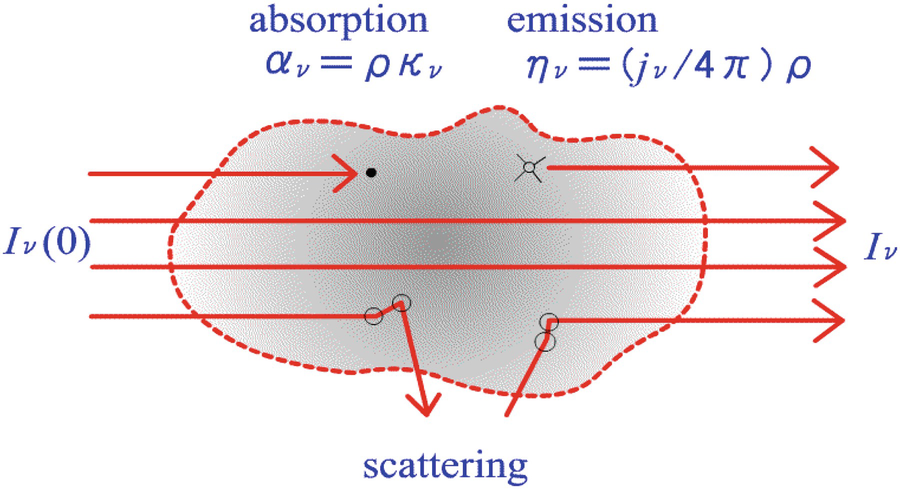
\includegraphics{Figures/radiative_transfer_scheme.png}
    \caption{Διάδοση ακτινοβολίας μέσα από ένα οπτικό μέσο. Ο παράγοντας $4\pi$ εμφανίζεται αν λάβουμε υπόψιν ότι ο συντελεστής επομπής (αφετική ικανότητα) $j_{\nu}$ ορίζεται ανά στερεά γωνία και ότι σε τοπική θερμοδυναμική ισορροπία, η εκπομπή ακτινοβολίας είναι ισοτροπική.}
    \label{fig:radiative_transfer_scheme}
\end{figure}


\subsubsection{Απορρόφηση \& Σκέδαση}
Θα προσπαθήσουμε να περιγράψουμε την μείωση στην ειδική ένταση της ακτινοβολίας κατά μήκος μια διαδρομής ds, στην κατεύθυνση $\boldsymbol{\hat{\eta}}$ λόγω της απορρόφησης της Η/Μ ακτινοβολίας από ένα οπτικό μέσο (σχήμα \ref{fig:radiative_transfer_scheme}). Στην περίπτωση που έχουμε ένα αδύναμο Η/Μ πεδίο και ένα αραιό οπτικό μέσο, τότε η μείωση της έντασης θα είναι ανάλογη της έντασης της εισερχόμενης ακτινοβολίας
\begin{equation}
    \label{eq:linear_absorption_coefficient}
    \frac{dI_{\nu}(\boldsymbol{\hat{\eta}})}{ds} \propto I_{\nu}(\boldsymbol{\hat{\eta}}) \longrightarrow \alpha_{\nu}(\boldsymbol{\hat{\eta}}) \left. \right|_{\rm absorption} \equiv - \frac{1}{I_{\nu}(\boldsymbol{\hat{\eta}})} \frac{dI_{\nu}(\boldsymbol{\hat{\eta}})}{ds}
\end{equation}
όπου ο συντελεστής αναλογίας $\alpha_{\nu}(\boldsymbol{\hat{\eta}}) \left. \right|_{\rm absorption}$, ονομάζεται \textit{γραμμικός συντελεστής απορρόφησης} και εκφράζει το κλάσμα της μονοχρωματικής ακτινοβολίας που αφαιρείται από την προσπίπτουσα δέσμη κατά μήκος μιας διεύθυνσης λόγω απορρόφησης.

Αντίστοιχα, μπορούμε να ορίσουμε και τον \textit{γραμμικό συντελεστή σκέδασης}, $\alpha_{\nu}(\boldsymbol{\hat{\eta}}) \left. \right|_{\rm scattering}$, ο οποίος εκφράζει το κλάσμα της μονοχρωματικής ακτινοβολίας ανά μονάδα μήκους που παρεκλίνει από την διεύθυνση, $\boldsymbol{\hat{\eta}}$, της προσπίπτουσας δέσμης λόγω σκέδασης. Έτσι, ορίζουμε τον \textit{γραμμικό συντελεστή απόσβεσης}
\begin{equation}
    \label{eq:linear_extinction_coefficient}
    \chi_{\nu} (\boldsymbol{\hat{\eta}}) \equiv \alpha_{\nu}(\boldsymbol{\hat{\eta}}) \left. \right|_{\rm absorption} + \alpha_{\nu}(\boldsymbol{\hat{\eta}}) \left. \right|_{\rm scattering}
\end{equation}
ο οποίος αναφέρεται στο συνολικό φαινόμενο της αφαίρεσης ειδικής έντασης από την προσπίπτουσα δέσμη ανά μονάδα μήκους. Από τη διαστασιακή ανάλυσης της σχέσης \eqref{eq:linear_absorption_coefficient}, προκύπτει ότι $$\left[\chi_{\nu} (\boldsymbol{\hat{\eta}})\right] = \left[\alpha_{\nu}(\boldsymbol{\hat{\eta}}) \left. \right|_{\rm absorption}\right] = \left[\alpha_{\nu}(\boldsymbol{\hat{\eta}}) \left. \right|_{\rm scattering}\right] = \left[L^{-1}\right]$$.

Το νόημα των μακροσκοπικών αυτών συντελεστών γίνεται εμφανές αν σκεφτούμε τι σημαίνει μείωση της έντασης της ακτινοβολίας σε μικροσκοπικό επίπεδο. Στην ατομική κλίμακα, η μείωση της έντασης οφείλεται στην αλληλεπίδραση των φωτονίων με ηλεκτρόνια, άτομα, μόρια ή ακόμα και μεγαλύτερες δομές που ονομάζουμε σκόνη. Ο συντελεστής απόσβεσης λοιπόν εξαρτάται από δύο παράγοντες: την πιθανότητα ένα φωτόνιο να απορροφηθεί ή να σκεδαστεί από κάποιο σωματίδιο, και τον αριθμό των ατόμων που περιέχονται σε έναν στοιχειώδη όγκο τα οποία είναι ικανά να απορροφήσουν ή να σκεδάσουν το εν λόγω φωτόνιο. 

Ο πρώτος παράγοντας, η πιθανότητα δηλαδή το φωτόνιο να αλληλεπιδράσει με κάποιο σωματίδιο, σχετίζεται με την \textbf{ενεργό διατομή} που είναι ο λόγος του αριθμού των φωτονίων που απορροφούνται/σκεδάζονται προς τη ροή των εισερχόμενων φωτονίων. Η ενεργός διατομή ενός σωματιδίου μπορεί να γίνει αντιληπτή αν θεωρήσουμε πως κάθε σωματίδιο ορίζει στον χώρο μία σφαίρα επιρροής, τέτοια ώστε η διέλευση ενός φωτονίου μέσα από αυτή να συνεπάγεται αλληλεπίδραση με το σωματίδιο. Το εμβδαδόν ενός μέγιστου κύκλου μιας τέτοιας σφαίρας, είναι η ενεργός διατομή του σωματιδίου, $\sigma_{\nu}$, η οποία γενικά εξαρτάται από τη συχνότητα και είναι μία ιδιότητα των σωματιδίων με διαστάσεις $[L^2]$. Ο δεύτερος παράγοντας, εκφράζεται από την αριθμητική πυκνότητα των σωματιδίων, $\eta$ και εξαρτάται από την θερμοδυναμική κατάσταση του οπτικού μέσου.

Είναι σαφές ότι εν γένει υπάρχουν πολλά σωματίδια το κάθε ένα από αυτά με τη δική του ενεργό διατομή για μια συγκεκριμένη διεργασία όπως η σκέδαση ή η απορρόφηση. Για λόγους απλότητας, ας υποθέσουμε ότι υπάρχει ένα μόνο είδος σωματιδίων ανά μονάδα όγκου και ότι κάθε ένα από αυτά έχει μία ενεργό διατομή για τη συλλογική απόσβεση της ακτινονολίας ίση με $\sigma_{\nu}$. Τότε, ο γραμμικός συντελεστής απόσβεσης θα ισούται 
\begin{equation}
    \label{eq:atomic_absorption_coefficient}
    \chi_{\nu} = \sigma_{\nu} \eta
\end{equation}
Από την παραπάνω έκφραση, βλέπουμε ότι ο γραμμικός συντελεστής απόσβεσης μπορεί να θεωρηθεί και ως ενεργός διατομή ανά μονάδα όγκου. Ισοδύναμα, μπορούμε να ορίσουμε τον γραμμικό συντελεστή απόσβεσης ως τη μείωση της έντασης της ακτινοβολίας ανά μονάδα μάζας (ή ενεργό διατομή ανά μονάδα μάζας), ώστε
\begin{equation}
    \label{eq:mass_extinction_coefficient}
    \chi_{\nu} = \kappa_{\nu} \rho
\end{equation}
όπου $\rho$ είναι η πυκνότητα μάζας του οπτικού μέσου με διαστάσεις $[M L^{-3}]$ και $\kappa_{\nu}$ ονομάζεται ο συντελεστής απόσβεσης μάζας (mass extinction coefficient) με διαστάσεις $[L^2 M^{-1}]$. Στην αστροφυσική, ο ορισμός ανά μονάδα μάζας είναι αυτός που χρησιμοποείται συνήθως στην μελέτη των αστρικών ατμοσφαιρών, με τον συντελεστή $\kappa_{\nu}$ να ονομάζεται \textbf{αδιαφάνεια} (opacity).

Βάσει των παραπάνω, η σχέση \eqref{eq:linear_absorption_coefficient} μπορεί να γραφτεί ισοδύναμα
\begin{equation}
    \label{eq:radiative_equation_extinction}
    \boxed{dI_{\nu} = - \chi_{\nu} I_{\nu} ds = - \sigma_{\nu} \eta I_{\nu} ds = - \kappa_{\nu} \rho I_{\nu} ds}
\end{equation}
και όπως έχουμε πει εκφράζει το πόσο μειώνεται η ειδική ένταση της ακτινοβολίας όταν διέρχεται από ένα οπτικό μέσο, σε σχέση με την αρχική ένταση.

Το αντίστροφο του μακροσκοπικού συντελεστή απόσβεσης συνδέεται με τη \textbf{μέση ελεύθερη διαδρομή}, $\ell$ , η οποία είναι η μέση απόσταση που διανύει ένα σωματίδιο σε ένα μέσο μεταξύ δύο διαδοχικών αλληλεπιδράσεων.
\begin{equation}
    \label{eq:mean_free_path}
    \ell \equiv \frac{1}{\chi_{\nu}} = \frac{1}{\sigma_{\nu} \eta} = \frac{1}{\kappa_{\nu} \rho}
\end{equation}

Εάν ο γραμμικός συντελεστής απόσβεσης μεταβάλλεται με την απόσταση, τότε το ολοκλήρωμα του γραμμικού συντελεστή απόσβεσης ως προς την απόσταση ορίζει ένα νέο (αδιάστατο) μέγεθος, το οποίο ονομάζουμε \textbf{οπτικό βάθος}, $\tau_{\nu}$
\begin{equation}
    \label{eq:optical_depth}
    \tau_{\nu} \equiv \int_{0}^{s} \chi_{\nu}(s^{\prime}) ds^{\prime} = \int_{0}^{s} \kappa_{\nu}(s^{\prime}) \rho(s^{\prime}) ds^{\prime} 
\end{equation}
και αποτελεί ένα μέτρο της "απορροφητικότητας" ενός οπτικού μέσου μέχρι ένα συγκεκριμένο βάθος.





\subsubsection{Εκπομή}
Έστω ένα μικρό στοιχείο όγκου $dV = dA ds$, όπου το $d$s έχει την ίδια διεύθυνση με τη διεύθυνση της δέσμης της ακτινοβολίας $\boldsymbol{\hat{\eta}}$, και η επιφάνεια $dA$ είναι κάθετη σε αυτή. Τότε η ενέργεια ανά μονάδα όγκου που προστίθεται στην αρχική δέσμη της ακτινοβολίας σε χρονικό διάστημα $dt$, με συχνοτικό εύρος $d\nu$ και μέσα σε μια στερεά γωνία $d\omega$ προς τη διεύθυνση $\boldsymbol{\hat{\eta}}$ της δέσμης θα είναι
\begin{equation}
    \label{eq:emission_coefficient}
    dE_{\nu}(\boldsymbol{\hat{\eta}}) = \eta_{\nu}(\boldsymbol{\hat{\eta}}) dt d\nu dA d\omega ds \longrightarrow dI_{\nu}(\boldsymbol{\hat{\eta}}) = \eta_{\nu}(\boldsymbol{\hat{\eta}}) ds
\end{equation}
όπου ο συντελεστής $\eta_{\nu}(\boldsymbol{\hat{\eta}})$ ονομάζεται (μονοχρωματικός) \textit{συντελεστής εκπομπής} του μέσου και στο σύστημα cgs έχει διαστάσεις $\rm \left[ erg \ s^{-1} \ Hz^{-1} \ cm^{-3} \ sr^{-1} \right]$. Επίσης, μπορούμε να ορίσουμε την ενέργεια που προστίθεται στην αρχική δέσμη ανά μονάδα μάζας με τη βοήθεια του συντελεστή \textit{αφετικής ικανότητας}, $j_{\nu}$ ώστε
\begin{equation}
    \label{eq:emissivity_coefficient}
    \eta_{\nu}(\boldsymbol{\hat{\eta}}) = j_{\nu}(\boldsymbol{\hat{\eta}}) \rho
\end{equation}
όπου $\rho$ είναι η πυκνότητα μάζας του μέσου. Η αφετική ικανότητα (emissivity) έχει διαστάσεις στο cgs $\rm \left[ erg \ s^{-1} \ Hz^{-1} \ sr^{-1} \ gr^{-1} \right]$. Με τη βοήθεια της σχέσης \eqref{eq:emissivity_coefficient}, μπορούμε να γράψουμε την εξίσωση \eqref{eq:emission_coefficient} ως
\begin{equation}
    \label{eq:radiative_equation_emission}
    \boxed{dI_{\nu}(\boldsymbol{\hat{\eta}}) = \eta_{\nu}(\boldsymbol{\hat{\eta}}) ds = j_{\nu}(\boldsymbol{\hat{\eta}}) \rho ds}
\end{equation}
όπου έχουμε θεωρήσει ότι ο συντελεστής εκπομπής (ή αφετική ικανότητα) συμπεριλαμβάνουν τη συνεισφορά στην αύξηση της ειδικής έντασης τόσο της αυθόρμητης εκπομπής όσο και της σκέδασης των φωτονίων από μία αρχική διεύθυνση $\boldsymbol{\hat{\eta}^{\prime}}$ στην διεύθυνση $\boldsymbol{\hat{\eta}}$ της δέσμης.

Συγκρίνοντας τις σχέσεις \eqref{eq:radiative_equation_extinction} και \eqref{eq:radiative_equation_emission} για την απόσβεση και εκπομπή ακτινοβολίας αντίστοιχα, παρατηρούμε ότι στην πρώτη περίπτωση η ενέργεια που αφαιρείται από τη δέσμη εξαρτάται από το πόσο ισχυρή ήταν η δέσμη αρχικά (αν δεν έχουμε καθόλου ενέργεια αρχικά τότε προφανώς τίποτα δεν μπορεί να αφαιρεθεί). Αντίθετα, η ενέργεια που προστίθεται στη δέσμη είναι ανεξάρτητη της έντασης. Η μόνη εξαίρεση σε αυτό αποτελεί η εξαναγκασμένη εκπομπή. Συνήθως αυτό το φαινόμενο αντιμετωπίζεται ως "αρνητική απορρόφηση" καθώς είναι εκπομπή που εξαρτάται από την ένταση της προσπίπτουσας ακτινοβολίας. Παρόλα αυτά, δεν θα ασχοληθούμε με αυτού του είδους τη συνεισφορά. 

Σε αυτό το σημείο μπορούμε να ορίσουμε τον λόγο 
\begin{equation}
    \label{eq:source_function}
    s_{\nu} \equiv \frac{\eta_{\nu}}{\chi_{\nu}} = \frac{j_{\nu}}{\kappa_{\nu}}
\end{equation}
ο οποίος ονομάζεται \textbf{συνάρτηση πηγής}\footnote{Οι περισσότεροι συγγραφείς αναφέρονται στη συνάρτηση πηγής με το σύμβολο $S_{\nu}$. Επειδή χρησιμοποιήσαμε το συγκεκριμένο σύμβολο για την πυκνότητα ροής, επιλέξαμε να χρησιμοποιήσουμε αντ' αυτού το πεζό σύμβολο $s_{\nu}$ προς αποφυγή σύγχησης.} (source function) και ουσιαστικά αποτελεί ένα μέτρο για το πόσα φωτόνια σε μία δέσμη αφαιρούνται και προστίθονται σε αυτή καθώς διέρχεται από ένα οπτικό μέσο. Οι διαστάσεις της συνάρτησης πηγής στο σύστημα cgs είναι $\rm \left[ erg \ s^{-1} \ Hz^{-1} \ cm^{-2} \ sr^{-1} \right]$, ίδιες δηλαδή με αυτές τις ειδικής έντασης.

Συνδυάζοντας τις σχέσεις \eqref{eq:radiative_equation_extinction}, \eqref{eq:radiative_equation_emission} και \eqref{eq:source_function}, προκύπτει ότι η διαφορική εξίσωση που περιγράφει τη διάδοση της ακτινοβολίας μέσα σε ένα οπτικό μέσο είναι
\begin{equation}
    \label{eq:radiative_transfer_equation}
    \frac{dI_{\nu}}{ds} = -\chi_{\nu} I_{\nu} + \eta_{\nu} =  - \kappa_{\nu} \rho I_{\nu} + j_{\nu} \rho
\end{equation}
ή χρησιμοποιώντας ισοδύναμα την έκφραση για το οπτικό βάθος (σχέση \eqref{eq:optical_depth})
\begin{eqnarray}
    \label{eq:radiative_transfer_equation_optical_depth_expressed}
    \frac{dI_{\nu}}{\kappa_{\nu} \rho ds} &=& - I_{\nu} + \frac{j_{\nu}}{\kappa_{\nu}} \Rightarrow  \boxed{\frac{dI_{\nu}}{d \tau_{\nu}} = s_{\nu} - I_{\nu}}
\end{eqnarray}



\subsubsection{Γενική λύση της εξίσωσης μεταφοράς}

{\color{red} \hrule} 
\textbf{Θεώρημα διαφορικών εξισώσεων}\\
Έστω μία μη-ομογενής γραμμική διαφορική εξίσωση της μορφής $$y^{\prime} + p(x) y = f(x)$$ 
Αν $y_h$ είναι μία μη-τετριμμένη (non-trivial) λύση της αντίστοιχης ομογενούς διαφορικής εξίσωσης $(f(x) = 0)$ και $y_p$ μία μερική (particular) λύση της μη-ομογενούς, τότε η γενική λύση της αρχικής διαφορικής εξίσωσης είναι $$y = y_h + y_p$$
όπου η μερική λύση $y_p$, σε αντίθεση με τη λύση $y_h$ της ομογενούς, \textit{δεν} περιέχει σταθερές.
{\color{red} \hrule} 

Η εξίσωση \eqref{eq:radiative_transfer_equation_optical_depth_expressed} είναι μία μη-ομογενής, γραμμική διαφορική εξίσωση πρώτου βαθμού της μορφής $$P_0 (x) y^{\prime} + P_1 (x) y = G(x), \hspace{1cm} G(x) \neq 0$$


\underline{\textit{Λύση της αντίστοιχης ομογενούς}}\\
Αν η συνάρτηση πηγής $s_{\nu} = 0$, τότε η εξίσωση μεταφοράς γράφεται
\begin{equation*}
    \frac{dI_{\nu}}{d\tau_{\nu}} + I_{\nu} = 0 \Rightarrow \frac{dI_{\nu}}{I_{\nu}} = - d\tau_{\nu} \Rightarrow \ln{I_{\nu}} + c = - \int_{0}^{\tau_{\nu}} d\tau^{\prime} 
\end{equation*}
ή
\begin{equation}
    \label{eq:homogeneous_DE_solution}
    I_{\nu} = \rm c e^{- \tau_{\nu}} = I_{\nu} (0) e^{- \tau_{\nu}}
\end{equation}
όπου για τον προσδιορισμό της σταθεράς $c$, χρησιμοποιήσαμε την αρχική συνθήκη $\tau_{nu} = 0 \longrightarrow I_{\nu} = I_{\nu} (0)$. Παρατηρούμε ότι η σχέση \eqref{eq:homogeneous_DE_solution} δεν είναι άλλη από τη γνωστή σχέση των Beer-Lambert.

Η λύση της ομογενούς εξίσωσης μεταφοράς είναι για την περίπτωση όπου η απόσβεση της ακτινοβολίας καθώς αυτή διέρχεται μέσα από ένα μέσο είναι σημαντική αλλά η εκπομπή ακτινοβολίας μπορεί να αγνοηθεί. 'Ενα τέτοιο παράδειγμα είναι η διάδοση φωτός μέσα από το διαστρικό μέσο (interstellar medium). Στα οπτικά μήκη κύματος, το διαστρικό μέσο δεν συνεισφέρει τίποτα στην ακτινοβολία καθώς η ύλη είναι πολύ ψυχρή. Η σκόνη όμως που παρεμβάλλεται μεταξύ της πηγής και του παρατηρητή μπορεί να προκαλέσει σημαντική απόσβεση της έντασης της ακτινοβολίας, αν το μήκος του μέσου είναι αρκετά μεγάλο.

\underline{\textit{Μερική λύση της μη-ομογενούς}}\\
Θα αναζητήζουμε λύσεις της μορφής $y_p(\tau_{\nu}) = u(\tau_{\nu}) y_h (\tau_{\nu})$, όπου $y_h$ είναι η μη-τετριμμένη λύση της ομογενούς (σχέση \eqref{eq:homogeneous_DE_solution}) και η $u(\tau_{\nu})$ πρέπει να προσδιοριστεί.
Η μέθοδος αυτή που στηρίζεται σε μια λύση της ομογενούς είναι γνωστή και ως "μεταβολή των σταθερών" (variation of parameters).

Εφόσον η $y_p (\tau_{\nu})$ είναι λύση της εξίσωσης μεταφοράς (σχέση \eqref{eq:radiative_transfer_equation_optical_depth_expressed}), θα πρέπει να την ικανοποιεί
\begin{eqnarray*}
    \frac{d}{d\tau_{\nu}} \left[ u(\tau_{\nu}) y_h (\tau_{\nu}) \right] + u(\tau_{\nu}) y_h (\tau_{\nu}) &=& s_{\nu} \Rightarrow \\\\
    \frac{du(\tau_{\nu})}{d \tau_{\nu}} y_h (\tau_{\nu}) + u(\tau_{\nu}) \frac{d y_h (\tau_{\nu})}{d \tau_{\nu}} + u(\tau_{\nu}) y_h(\tau_{\nu}) &=& s_{\nu} \Rightarrow \\\\
    \frac{d u(\tau_{\nu})}{d \tau_{\nu}} I_{\nu}(0) \rm e^{- \tau_{\nu}} - \cancel{u(\tau_{\nu}) I_{\nu}(0) e^{-\tau_{\nu}}} + \cancel{u(\tau_{\nu}) I_{\nu}(0) \rm e^{- \tau_{\nu}}} &=& s_{\nu} \Rightarrow \\\\
    \frac{d u(\tau_{\nu})}{d \tau_{\nu}} = \frac{s_{\nu}}{I_{\nu}(0)} \rm e^{\tau_{\nu}} \Rightarrow u(\tau_{\nu}) &=& \int_{0}^{\tau_{\nu}} \frac{s_{\nu}}{I_{\nu}(0)} \rm e^{\tau^{\prime}} d \tau^{\prime} 
\end{eqnarray*}

Άρα. η μερική λύση της μη-ομογενούς εξίσωσης μεταφοράς είναι
\begin{eqnarray}
    \label{eq:inhomogeneous_DE_solution}
    y_p (\tau_{\nu}) &=& u(\tau_{\nu}) y_h (\tau_{\nu}) = \cancel{I_{\nu}(0)} \rm e^{- \tau_{\nu}} \int_{0}^{\tau_{\nu}} \frac{s_{\nu}}{\cancel{I_{\nu}(0)}} \rm e^{\tau^{\prime}} d \tau^{\prime} \Rightarrow \nonumber \\ \nonumber \\
    &\Rightarrow & y_p (\tau_{\nu}) = \int_{0}^{\tau_{\nu}} s_{\nu} \rm e^{\tau^{\prime} - \tau_{\nu}} d \tau^{\prime}
\end{eqnarray}

Τελικά, συνδυάζοντας τις λύσεις \eqref{eq:homogeneous_DE_solution} και \eqref{eq:inhomogeneous_DE_solution}, καταλήγουμε ότι η γενική λύση της εξίσωσης μεταφοράς είναι
\begin{equation}
    \label{eq:radiative_transfer_general_solution}
    \boxed{I_{\nu} (\tau_{\nu}) = I_{\nu} (0) \rm e^{- \tau_{\nu}} + \int_{0}^{\tau_{\nu}} s_{\nu} \rm e^{\tau^{\prime} - \tau_{\nu}} d \tau^{\prime}}
\end{equation}
όπου ο πρώτος όρος μας λέει ότι η ένταση της αρχικής δέσμης μειώθηκε κατά έναν παράγοντα $\rm e^{\tau_{\nu}}$ λόγω απόσβεσης. Όμως ένα οπτικό μέσο μπορεί να εκπέμπει και αυτό ακτινοβολία η ένταση της οποίας υπόκειται και αυτή σε απορρόφηση ή σκέδαση στη θέση $\tau^{\prime}$. Αυτή η διαδικασία περιγράφεται από τον δεύτερο όρο της λύσης της εξίσωσης μεταφοράς.

Επιπροσθέτως, εαν η συνάρτηση πηγής είναι ανεξάρτητη της θέσης μέσα στο οπτικό μέσο, μπορεί να βγει έξω από το ολοκλήρωμα της σχέσης \eqref{eq:radiative_transfer_general_solution}. Τότε η λύση της εξίσωσης μεταφοράς μπορεί να γραφτεί με την απλοποιημένη μορφή
\begin{equation}
    \label{eq:radiative_transfer_simple_solution}
    \boxed{I_{\nu}(\tau_{\nu}) = I_{\nu} (0) \rm e^{- \tau_{\nu}} + s_{\nu} \left( 1 - \rm e^{- \tau_{\nu}} \right)}
\end{equation}

Για να γίνει αντιληπτή η φυσική σημασία της λύσης \eqref{eq:radiative_transfer_simple_solution}, θα εξετάσουμε τις ακόλουθες οριακές περιπτώσεις

\begin{itemize}
    \item Όταν $\tau_{\nu} = 0$, σημαίνει ότι είτε δεν υπάρχει καθόλου ύλη, οπότε $\rho = 0$, είτε η ύλη είναι εντελώς διαφανής σε ακτινοβολίας συχνότητας $\nu$, οπότε $\kappa_{\nu} = 0$. Τότε, η λύση της εξίσωσης μεταφοράς μας δίνει ότι $$I_{\nu} = I_{\nu}(0)$$ πράγμα που σημαίνει ότι ο παρατηρητής βλέπει μόνο την ακτινοβολία της πηγής. Τότε ο ορισμός της συνάρτησης πηγής του οπτικού μέσου (αν υπάρχει) είναι δυνατό να ικανοποιείται μόνο αν $j_{\nu} = 0$. Ένα εντελώς διάφανο μέσο λοιπόν δεν εκπέμπει καθόλου ακτινοβολία.
    \item Στην περίπτωση που $\tau_{\nu} \gg 1$, τότε τα εκθετικά στη σχέση \eqref{eq:radiative_transfer_simple_solution} είναι προσεγγιστικά ίσα με μηδέν, και η λύση της εξίσωσης μεταφοράς γράφεται $$I_{\nu} = s_{\nu}$$ πράγμα που σημαίνει ότι ο παρατηρητής βλέπει μόνο την επιφάνεια του οπτικού μέσου και δεν βλέπει καθόλου την φωτεινή πηγή πίσω από αυτό (δες και σχήμα \ref{fig:optical_depth_examples}). Το οπτικό μέσο δηλαδή είναι τελείως αδιαφανές και χαρακτηρίζεται ως "οπτικά παχύ" (optically thick).
    Στην αντίθετη περίπτωση, δηλαδή όταν $\tau_{\nu} \ll 1$, τότε λέμε ότι το μέσο είναι \textit{οπτικά λεπτό} (optically thin) και υπάρχει μικρή απόσβεση της ακτινοβολίας.
    \item Τέλος, αν $\tau_{\nu} \approx 1$, τότε η φωτεινή ένταση που φτάνει στον παρατηρητή οφείλεται και στην πηγή και στο οπτικό μέσο και η λύση της εξίσωσης μεταφοράς είναι $$I_{\nu} = 0.368 I_{\nu}(0) + 0.632 s_{\nu}$$
\end{itemize}

\begin{figure}
    \centering
    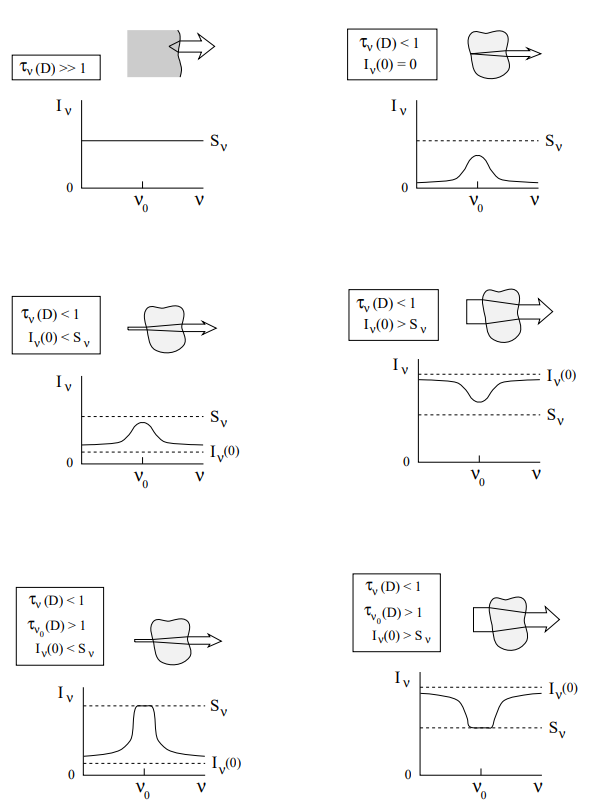
\includegraphics[width=\textwidth]{Figures/optical_depth_examples.png}
    \caption{Φασματικές γραμμές από ένα ομοιογενές οπτικό μέσο με συνάρτηση πηγής $s_{\nu}$. Καμία γραμμή δεν εμφανίζεται όταν το μέσο είναι οπτικά παχύ (πάνω αριστερά). Όταν είναι οπτικά λεπτό, εμφανίζονται γραμμές εκπομπής όταν δεν υπάρχει πηγή ακτινοβολίας από πίσω ($I_{\nu}(0) = 0$, πάνω αριστερά), ή όταν προσπίπτει ακτινοβολία με $I_{\nu}(0) < s_{\nu}$. Γραμμές απορρόφησης εμφανίζονται μόνο όταν το μέσο είναι οπτικά λεπτό και ακτινοβολείται από δέσμη με ένταση $I_{\nu}(0) > s_{\nu}$. Οι εμφανιζόμενες γραμμές εμφανίζουν κορεσμό στο $I_{\nu} \approx s_{\nu}$ όταν το μέσο είναι οπτικά παχύ στη συχνότητα $\nu_0$.}
    \label{fig:optical_depth_examples}
\end{figure}


\subsection{Νόμος του Kirchhoff}
{\color{red} \hrule}
Ο νόμος της φασματοσκοπίας του Kirchhoff συνδέει το ρυθμό εκπομπής ακτινοβολίας ενός σώματος σε θερμοδυναμική ισορροπία με το ρυθμό απορρόφησης της ακτινοβολίας από το ίδιο σώμα.\\
{\color{red} \hrule}

Η φυσική σημασία της συνάρτησης πηγής $s_{\nu}$ γίνεται φανερή, αν υποθέσουμε ότι το οπτικό μέσο βρίσκεται σε θερμοδυναμική ισορροπία, δηλαδή ύλη και ακτινοβολία χαρακτηρίζονται από την ίδια θερμοκρασία $T$. Τότε η ένταση της ακτινοβολίας $I_{\nu}$ εξ' ορισμού δεν μεταβάλλεται στο εσωτερικο του μέσου, δηλαδή όσο ακτινοβολία απορροφάται σε κάθε σημείο του εσωτερικού του, τόση και εκπέμπεται. Στην περίπτωση αυτή $dI_{\nu}/ds = 0$, οπότε από τη σχέση \eqref{eq:radiative_transfer_equation} προκύπτει ότι 
\begin{equation}
    I_{\nu} = s_{\nu} = B_{\nu} (T) = \frac{2h \nu^3}{c^2} \frac{1}{\exp \left( \frac{h \nu}{kT} \right) - 1}
\end{equation}

Η τελευταία ισότητα της παραπάνω σχέσης ισχύει καθώς αφού το πεδίο ακτινοβολίας βρίσκεται σε θερμοδυναμική ισορροπία, εξαρτάται μόνο από τη θερμοκρασία του οπτικού μέσου και όχι από οποιαδήποτε άλλη φυσική ιδιότητά του, και η ένταση του θα δίνεται από τον νόμο του Planck. Με άλλα λόγια, στην περίπτωση που το οπτικό μέσο βρίσκεται σε θερμοδυναμική ισορροπία, η συνάρτηση πηγής είναι ανεξάρτητη από το υλικό του οπτικού μέσου και ισούται με την ένταση της ακτινοβολίας μέλανος σώματος. Αυτή η πρόταση αποτελεί το \textit{νόμο της φασματοσκοπίας του Kirchhoff}. 


\section{Αδιαφάνεια και αστρικά φάσματα}
Όπως αναφέραμε και προηγουμένως, οι μικροφυσικοί μηχανισμοί των οποίων το αποτέλεσμα εκφράζεται φαινομενολογικά ως συντελεστής απόσβεσης και εκπομπής, είναι κατά βάση κβαντικά φαινόμενα, αφού σχετίζονται με απορρόφηση, σκέδαση, και εκπομπή φωτονίων. Τα κύρια κβαντικά φαινόμενα που αποτελούν πηγές αδιαφάνειας στην Αστρονομία είναι οι μεταπτώσεις ηλεκτρονίων και μορίων από μία ενεργειακή κατάσταση σε μία άλλη. Επειδή οι μοριακές μεταπτώσεις είναι σημαντικές μόνο σε χαμηλές θερμοκρασίες, όπως π.χ. στις ατμόσφαιρες των ψυχρότερων αστέρων και στα νεφελώματα, η αδιαφάνεια που οφείλεται σε τέτοιου είδους μεταπτώσεις δεν θα μας απασχολήσει σε αυτό το επίπεδο.

\subsection{Μηχανισμοί αδιαφάνειας}
 Οι ηλεκτρονικές μεταπτώσεις που είναι υπεύθυνες για την αστρική αδιαφάνεια οφείλονται σε τέσσερις βασικούς μηχανισμούς:
\begin{enumerate}
    \item \textbf{Μεταπτώσεις από δέσμια σε ελεύθερη κατάσταση (bound-free transition ή φωτοϊονισμός) ή από ελεύθερη σε δέσμια κατάσταση (επανασύνδεση ή recombination)} 
    
    Η περίπτωση της επανασύνδεσης αναφέρεται στην σύγκρουση και απορρόφηση ενός ηλεκτρονίου με ένα ιόν, εκπέμποντας ένα φωτόνιο κατά τη διαδικασία αυτή. Η ενέργεια αυτού του φωτονίου θα ισούται με την κινητική ενέργεια του ηλεκτρονίου συν την ενέργεια σύνδεσης του ηλεκτρονίου που πλέον είναι μέρος του ιόντος. Επειδή η κινητική ενέργεια που είχε το ηλεκτρόνιο δεν οφείλει να είναι κβαντισμένη, η μετάπτωση επανασύνδεσης αποτελεί πηγή συνεχούς αδιαφάνειας (continuum spectrum). Παρόμοια λογική ισχύει και για την περίπτωση της δέσμιας-ελεύθερης μετάπτωσης.
    
    \item \textbf{Μεταπτώσεις από ελεύθερη σε ελεύθερη κατάσταση με την παρουσία ατομικών πυρήνων (free-free transition ή Bremsstrahlung)}
    
    Η ακτινοβολία πέδησης όπως αποκαλείται οφείλεται σε επιβράδυνση των ηλεκτρονίων (ή οποιουδήποτε φορτίου) τα οποία σκεδάζονται από άλλα άτομα ή ιόντα, χωρίς να συλλαμβάνονται από αυτά. Αυτή η διαδικασία αποτελεί ακόμα μία πηγή συνεχούς αδιαφάνειας.
    
    \item \textbf{Μεταπτώσεις από ελεύθερη σε ελεύθερη κατάσταση λόγω σκεδασμού φωτονίων από ηλεκτρόνια (σκέδαση Thomson και φαινόμενο Compton)}
    
    Στην σκέδαση Thomson, ένα φωτόνιο σκεδάζεται ελαστικά από ένα φορτισμένο σωματίδιο (συνήθως ηλεκτρόνιο) χωρίς να αλλάζει η κινητική ενέργεια του σωματιδίου ούτε η συχνότητα του φωτονίου. Η σκέδαση Thomson αποτελεί το όριο χαμηλών ενεργείων του πιο γενικού φαινομένου Compton.
    
    Στη σκέδαση Compton, ένα φωτόνιο σκεδάζεται από ένα φορτισμένο σωματίδιο (συνήθως ηλεκτρόνιο) με αποτέλεσμα να μειωθεί η ενέργειά του (να αυξηθεί το μήκος κύματος). Μέρος της ενέργειας του φωτονίου μεταφέρεται στο ανακρουόμενο ηλεκτρόνιο. Το αντίστροφο φαινόμενο Compton λαμβάνει χώρα όταν ένα φορτισμένο σωματίδιο μεταφέρει μέρος της ενέργειάς του σε ένα φωτόνιο.
    
    Καθώς και τα δύο αυτά φαινόμενα σκέδασης περιλαμβάνουν ελεύθερα σωματίδια, αποτελούν πηγές συνεχούς αδιαφάνειας.
    
    \item \textbf{Μεταπτώσεις από δέσμια σε δέσμια κατάσταση (διέγερση ατόμων ή ιόντων)}
    Η μετάπτωση από κάποια ενεργειακή στοιβάδα σε μία άλλη ενεργειακή στοιβάδα θα παράξει φωτόνιο καθορισμένης ενέργειας και άρα αυτού του είδους η μετάπτωση δεν αποτελεί πηγή συνεχούς αδιαφάνειας.
\end{enumerate}

Είναι φανερό ότι οι μηχανισμοί 1-3 προϋποθέτουν την ύπαρξη ελεύθερων ηλεκτρονίων και ιονισμένων ατόμων σε σημαντικές αριθμητικές πυκνότητες, γεγονός που προϋποθέτει υψηλές θερμοκρασίες. Δεδομένου ότι η ενέργεια ιονισμού του Υδρογόνου είναι $\rm 13.6 \ eV$, η θερμοκρασία που πρέπει να επικρατεί είναι της τάξης των $\rm 11600 \ K$. Τέτοιες θερμοκρασίες συναντώνται κατ' εξοχήν στο εσωτερικό των αστέρων  και στις επιφάνειες αστέρων προγενέστερου φασματικού τύπου. 

Ο τέταρτος μηχανισμός προϋποθέτει την ύπαρξη ουδέτερων ατόμων, που ακολουθώντας την ίδια συλλογιστική, μας οδηγεί στο συμπέρασμα ότι είναι κατ' εξοχήν σημαντικός στην επιφάνεια των αστέρων (φωτόσφαιρα) και στην ατμόσφαιρα των αστέρων, εκεί δηλαδή όπου παράγεται το συνεχές φάσμα και οι φασματικές γραμμές απορρόφησης (και ενδεχομένως εκπομπής) των αστέρων.

\subsection{Η συνεχής συνιστώσα}
Τόσο το συνεχές όσο και το γραμμικό φάσμα, δημιουργούνται ταυτόχρονα σε όλο το βάθος των εξωτερικών στρωμάτων ενός αστέρα, από τη φωτόσφαιρα μέχρι την κορυφή της ατμόσφαιρας.
Από τον νόμο του Kirchhoff, γνωρίζουμε ότι ένα σώμα που εκπέμπει συνεχές φάσμα πρέπει να έχει κάποια πηγή συνεχούς αδιαφάνειας. Οι τρεις πρώτες περιπτώσεις που αναφέραμε παραπάνω αποτελούν παραδείγματα τέτοιων μηχανισμών, και επομένως καθεμία από αυτές θα μπορούσε να είναι υπεύθυνη για τη συνεχή εκπομπή. Επειδή τα αστέρια αποτελούνται κατά βάση από Υδρογόνο και Ήλιο, η ασυνεχής αδιαφάνεια θα πρέπει να είναι συνδεδεμένη με τον ιονισμό του Υδρογόνου ή/και του Ηλίου στην επιφάνεια των αστέρων. Όμως ο ιονισμός του Υδρογόνου απαιτεί θερμοκρασίες άνω των $\rm 10000 \ K$, όπως έχουμε αναφέρει, ενώ ο ιονισμός του Ηλίου ακόμα μεγαλύτερες θερμοκρασίες. Τέτοιες θερμοκρασίες συναντώνται πραγματικά στις ατμόσφαιρες των αστέρων προγενέστερου φασματικού τύπου αλλά όχι και στις ψυχρότερες ατμόσφαιρες των αστέρων μεταγενέστερου φασματικού τύπου, όπως ο Ήλιος.

Σήμερα γνωρίζουμε ότι κύρια πηγή αδιαφάνειας στην ατμόσφαιρα του Ήλιου είναι ο φωτοϊονισμός, αλλά όχι στη συνηθισμένη εκδοχή του. Είναι η μετάπτωση από δέσμια σε ελεύθερη κατάσταση του επιπλέον ηλεκτρονίου του \textit{αρνητικού ιόντος} του Υδρογόνου $\rm H^{-}$
$$\rm H^{-} + h\nu \leftrightharpoons H + e^{-}$$
Αυτή η διαδικασία αναφέρεται ως "φωτοδιάσπαση" γιατί δίνει ένα ουδέτερο άτομο αντί για ένα ιόν. Επομένως, όταν το ανιόν του Υδρογόνου διασπάται, απορροφά φωτόνια συνεχούς ενέργειας, και άρα είναι πηγή συνεχούς αδιαφάνειας, ενώ όταν συντίθεται εκπέμπει φωτόνια συνεχούς ενέργειας και άρα είναι πηγή συνεχούς εκπομπής.

Το $\rm H^{-}$ έχει ενέργεια σύνδεσης $\rm 0.75 \ eV$ που αντιστοιχεί σε θερμοκρασία περίπου $\rm 8700 \ K$. Άρα, σε αστέρες με ενεργό θερμοκρασία μικρότερη από $\rm 8700 \ K$ η δημιουργία του $\rm H^{-}$ ευνοείται θερμοδυναμικά καθώς η δέσμια κατάσταση είναι κατά $\rm 0.75 \ eV$ ενεργειακά μικρότερη από την ενέργεια ηρεμίας ενός ατόμου Υδρογόνου και ενός ελεύθερου ηλεκτρονίου. Αντίθετα, σε αστέρες με ενεργό θερμοκρασία μεγαλύτερη από $\rm 8700 \ K$ η δημιουργία του $\rm H^{-}$ δεν ευνοείται καθώς πάρα πολλά φωτόνια έχουν ενέργεια μεγαλύτερη από $\rm 0.75 \ eV$ και προκαλούν ανισορροπία στις αντιδράσεις σχηματισμού-καταστροφής του $\rm H^{-}$, ευνοώντας τις τελευταίες. Είναι προφανές, πως αν η αριθμητική πυκνότητα των ιόντων $\rm H^{-}$ είναι μικρή, τότε η συμμετοχή τους στην παραγωγή της συνεχούς συνιστώσας του φάσματος εκπομπής είναι αμελητέα.

Αυτός ο μηχανισμός εξηγεί την δημιουργία του συνεχούς φάσματος του Ήλιου μόνο για τα μήκη κύματος για τα οποία ισχύει η σχέση $\rm h\nu > 0.75 \ eV$, τα οποία περιλαμβάνουν το ορατό φάσμα και το εγγύς υπέρυθρο. Η ένταση της συνεχούς ακτινοβολίας του Ήλιου τα ραδιοφωνικά μήκη κύματος, μέρος του υπεριώδους και στις ακτίνες Χ ειναι πολύ μεγαλύτερη από αυτή που προβλέπει ο νόμος του Planck και δεν μπορεί να εξηγηθεί με τον παραπάνω μηχανισμό. Αυτό συμβαίνει γιατί η ακτινοβολία στις συγκεκριμένες συχνοτικές περιοχές, δεν είναι θερμικής φύσης δηλαδή προέρχονται από υλικό που δεν είναι σε θερμοδυναμική ισορροπία, και επομένως δεν ισχύει στην περίπτωση αυτή ούτε ο νόμος του Planck, ούτε ο νόμος του Kirchhoff.



\section{Νόμοι Boltzmann \& Saha}
\subsection{Νόμος του Boltzmann}
Η κατανομή των ατόμων ενός στοιχείου (ουδέτερων ή ιονισμένων) στις διάφορες ενεργειακές στάθμες ακολουθεί τη στατιστική Maxwell-Boltzmann, είναι συνάρτηση της απόλυτης θερμοκρασίας $T$ της ατμόσφαιρας και δίνεται από τον νόμο του Boltzmann\footnote{Δες Παράρτημα \ref{apx:kinetic_theory} για απόδειξη της σχέσης.}
\begin{eqnarray}
    \label{eq:boltmann_law}
    \frac{n_{i,j}}{n_{0,j}} = \frac{g_{i,j}}{g_{0,j}} e^{-E_i/(kT)}
\end{eqnarray}
όπου η τιμή 0 υποδηλώνει τη θεμελιώδη στάθμη του ατόμου. Η μεταβλητή $n_{i,j}$ παριστάνει την αριθμητική πυκνότητα (αριθμός ατόμων ανά $\rm cm^3$) των ατόμων που είναι διεγερμένα στη στάθμη i $(i=0,1,\dots)$ και βρίσκονται στην κατάσταση ιονισμού j ($j = 0$ για ουδέτερα άτομα, $j=1$ για απλά ιονισμένα κτλ). Η μεταβλητή $E_i$ είναι η ενέργεια διέγερσης από τη στάθμη 0 στη στάθμη i, και k είναι η σταθερά του Boltzmann. Τέλος, $g_{i,j}$ είναι η πολλαπλότητα (ή στατιστικό βάρος) της στάθμης i, και παριστάνει το πλήθος των ενεργειακών υποσταθμών της στάθμης i υπό την παρουσία μαγνητικού πεδίου (δες φαινόμενο Zeeman). Ο συντελεστής $g_{i,j}$ συνδέεται με την ολική στροφορμή J του ατόμου με τη σχέση 
\begin{eqnarray}
    \label{eq:total_angular_momentum}
    g_{i,j} = 2J + 1
\end{eqnarray}

Ειδικά για το άτομο του Υδρογόνου ισχύει $$g_{i,0} = g_i = 2(i+1)^2 \ i = 0,1,\dots$$ αφού ο δείκτης j δεν μπορεί να πάρει τιμή διάφορη του 0 (το Υδρογόνο έχει ένα μόνο ηλεκτρόνιο και, αν ιονισθεί, δεν υπάρχει άλλο έτσι ώστε οι αλλαγές των κβαντικών αριθμών του οποίου να αλλάζουν την κβαντική κατάσταση του ιόντος του Υδρογόνου).

Είναι φανερό ότι το άθροισμα

\begin{equation}
    \label{eq:number_density_of_atoms_in_j_state}
    n_j = \sum_{i=0}^{\infty} n_{i,j} = \frac{n_{0,j}}{g_{0,j}} \sum_{i=0}^{\infty} g_{i,j} e^{-E_i/(kT)} = \frac{n_{0,j}}{g_{0,j}} Z_j(T)
\end{equation}
όπου $Z_j(T)$ η συνάρτηση επιμερισμού. Η σχέση \eqref{eq:number_density_of_atoms_in_j_state} παριστάνει την αριθμητική πυκνότητα των ατόμων που βρίσκονται στην κατάσταση ιονισμού j, ανεξάρτητα από τη στάθμη διέγερσης.

Διαιρώντας κατά μέλη τις σχέσεις \eqref{eq:boltmann_law} και \eqref{eq:number_density_of_atoms_in_j_state}, προκύπτει ο νόμος του Boltzmann στη συνηθισμένη μαθηματική μορφή του
\begin{equation}
    \label{eq:boltzmann_law_general}
    \frac{n_{i,j}}{n_j} = \frac{g_{i,j}}{Z_{j}(T)} e^{-E_i/(kT)}
\end{equation}
η οποία δίνει το λόγο της αριθμητικής πυκνότητας των ατόμων ενός στοιχείου, σε μια συγκεκριμένη κατάσταση διέγερσης και ιονισμού, προς την αριθμητική πυκνότητα των ατόμων του ίδιου στοιχείου, στην ίδια κατάσταση ιονισμού, ανεξάρτητα από την κατάσταση διέγερσης. Ο παράγοντας $e^{-E_i/(kT)}$ ονομάζεται και παράγοντας Boltzmann.



\subsection{Νόμος του Saha}
Η συναρτησιακή μορφή της σχέσης που μας δίνει τα ποσοστά των ιονισμένων ατόμων μπορεί να υπολογισθεί από τις βασικές αρχές των νόμων της χημικής ισορροπίας. Αν η ύλη στην ατμόσφαιρα του αστέρα βρίσκεται σε θερμοδυναμική ισορροπία, τότε ο ρυθμός του (απλού) ιονισμού των ατόμων ενός στοιχείου είναι ίσος με το ρυθμό επανασύνδεσής τους. Αυτή η κατάσταση παριστάνεται συμβολικά με τη χημική εξίσωση $$\text{A} + h\nu \leftrightharpoons \text{A}^+ + e^-$$ όπου $\text{A}$, $\text{A}^+$ και $e^-$ παριστάνουν αντίστοιχα το ουδέτερο άτομο, το ιονισμένο άτομο και το ηλεκτρόνιο. Ας υποθέσουμε ότι $N_0, N_i, N_e$ είναι ο αριθμός των ουδέτερων ατόμων, των ιονισμένων ατόμων και των ηλεκτρονίων αντίστοιχα, τα οποία βρίσκονται σε ένα κουτί όγκου $V$. Τότε, η εξίσωση του Saha θα είναι:
\begin{equation}
    \label{eq:saha_function}
    \frac{N_e N_i}{N_0} = S (T,P)
\end{equation}

Η εξίσωση του Saha είναι συνάρτηση της πίεσης και της θερμοκρασίας, με την υψηλή θερμοκρασία να ευνοεί τον ιονισμό ενώ η υψηλή πίεση την επανασύνδεση (recombination). Η εξίσωση μας λέει ότι οι σχετικοί αριθμοί τριών τύπων σωματιδίων (με άλλα λόγια ο βαθμός ιονισμού) σε μια κατάσταση ισορροπίας, όταν ο ρυθμός ιονισμού είναι ίσος με τον ρυθμό επανασύνδεσης.

Γνωρίζουμε ότι ο αριθμός των σωματιδίων σε ένα συγκεκριμένο ενεργειακό επίπεδο είναι ανάλογος του παράγοντα Boltzmann για το συγκεκριμένο επίπεδο, και ο ολικός αριθμός των σωματιδίων είναι ανάλογος του αθροίσματος των παραγόντων Boltzmann για όλα τα ενεργειακά επίπεδα --- δηλαδή, ανάλογος της συνάρτησης επιμερισμού. Έτσι, η εξίσωση του Saha γράφεται

\begin{equation}
    \label{eq:saha_partition_functions}
    \frac{N_e N_i}{N_0} = \frac{Q_e Q_i}{Q_0}
\end{equation}

Όπως είπαμε, η συνάρτηση επιμερισμού είναι το άθροισμα όλων των παραγόντων Boltzmann για όλες τις ενεργειακές καταστάσεις, μεταφορικές (χωρίς περιστροφή) και εσωτερικές (ηλεκτρονιακή δομή). Η ολική ενέργεια ενός σωματιδίου είναι το άθροισμα της μεταφορικής και εσωτερικής ενέργειας, έτσι ώστε η ολική συνάρτηση επιμερισμού να είναι το γινόμενο των μεταφορικών και εσωτερικών συναρτήσεων επιμερισμού\footnote{Δες σχετικό κεφάλαιο στο Παράρτημα \ref{apx:kinetic_theory}}, για τις οποίες θα χρησιμοποιήσουμε το σύμβολο $u$. Έτσι έχουμε:
\begin{equation}
    \frac{N_e N_i}{N_0} = \left( \frac{2\pi m k T}{h^2} \right)^{\frac{3}{2}} V \frac{u_e u_i}{u_0}
\end{equation}
όπου $m = \frac{m_e m_i}{m_0}$, και διαφέρει πολύ λίγο από το $m_e$.

Η εσωτερική συνάρτηση επιμερισμού του ηλεκτρονίου ισούται με το στατιστικό του βάρος $2s + 1 = 2$. 'Ετσι, μπορούμε να γράψουμε την παραπάνω εξίσωση με όρους αριθμητικής πυκνότητας $(n = N/V)$ και να καταλήξουμε στη συνηθισμένη μορφή της εξίσωσης του Saha:
\begin{equation}
    \label{eq:saha_equation_full}
    \frac{n_e n_i}{n_0} = \left( \frac{2\pi m k T}{h^2} \right)^{\frac{3}{2}} \frac{2u_i}{u_0} \exp \left( - \frac{\chi_i}{kT} \right)
\end{equation}
όπου $\chi_i$ είναι η ενέργεια ιονισμού.

Η εξίσωση Saha έπεξε καθοριστικό ρόλο στην κατανόηση των αστρικών φασμάτων. Όπως έχουμε αναφέρει, η φασματική ταξινόμηση $\text{O,B,A,F,G, \dots}$ είναι αποτέλεσμα του βαθμού ιονισμού και διέγερσης των χημικών στοιχείων ως συνάρτηση της θερμοκρασίας, ενώ η διαφορά στο βαθμό ιονισμού μεταξύ αστέρων της κύριας ακολουθίας και αστέρες-γίγαντες μιας συγκεκριμένης θερμοκρασίας είναι το αποτέλεσμα του υψηλότερου βαθμού ιονισμού στις σχετικά χαμηλής πίεσης ατμόσφαιρες των αστέρων-γιγάντων.



\section{Ο Ήλιος ως τυπικός αστέρας}
\subsection{Μακροσκοπικά χαρακτηριστικά}
Από τις παρατηρήσεις που έχουμε για τον Ήλιο, γνωρίζουμε πως η φαινόμενη διάμετρός του είναι
$$d = 32^\prime = 9.3 \times 10^{-3} \hspace{0.5cm} \text{rad}$$ που αντιστοιχεί σε ακτίνα
$$R_{\odot} = 1 \ \text{AU} \times \sin{\frac{d}{2}} = 6.96 \times 10^{10} \hspace{0.25cm} \text{cm}$$ και η οποία είναι σε γενικές γραμμές σταθερή (πέρα από μερικές μικρές ταλαντώσεις). Η βολομετρική φαινόμενη λαμπρότητα του Ήλιου, δηλαδή η ολική φωτεινή ροή της ακτινοβολίας του Ήλιου σε απόσταση 1 AU ονομάζεται \textbf{ηλιακή σταθερά}, $f$, και ισούται με 
$$f=1.36 \times 10^6 \hspace{0.25cm} \text{erg sec$^{-1}$ cm$^{-2}$}$$

Υποθέτωντας πως ο Ήλιος ακτινοβολεί ισοτροπικά, η ηλιακή σταθερά ισούται με τη λαμπρότητα του Ήλιου (δηλαδή την ισχύ που ακτινοβολεί σε όλο το εύρος του ηλεκτρομαγνητικού φάσματος) διαμοιρασμένη στην επιφάνεια μιας σφαίρας με ακτίνα την αστρονομική μονάδα
$$L_{\odot} = 4\pi f (1 \ \text{AU})^2 = 3.9 \times 10^{33} \hspace{0.25cm} \text{erg sec$^{-1}$}$$
Η ενεργός θερμοκρασία του Ήλιου, όπως υπολογίζεται με τη βοήθεια της σχέσης
$$L_{\odot} = 4\pi R^2 \sigma T_{\text{eff}}^4$$ 
είναι $T_{\text{eff}} = 5800 \hspace{0.25cm} \text{K}$, ο δε φασματικός τύπος του \textbf{G2V}.

Η μάζα του Ήλιου μπορεί να υπολογιστεί είτε από τον τρίτο νόμο του Kepler 
$$\frac{A^3}{P^3} = G \frac{M_{\odot} + M_{\oplus}}{4 \pi ^2}$$ αν θέσουμε $A = 1 \ AU$, $P = 1 \ \text{yr}$ και αγνοήσουμε τη μάζα της Γης σε σύγκριση με τη μάζα του Ήλιου, θέτοντας $M_{\oplus} = 0$. Έτσι βρίσκουμε $M_{\odot} \simeq 2 \times 10^{33} \hspace{0.25cm} \text{gr}$. Ένας άλλος τρόπος είναι από την περιφορά της Γης γύρω από τον Ήλιο αν εξισώσουμε την κεντρομόλο δύναμη με την δύναμη της βαρύτητας:
$$F = ma \Rightarrow G \frac{M_\odot M_\oplus}{d^2} = M_\oplus \frac{v^2}{d} \Rightarrow M_{\odot} = \frac{v^2 d}{G}$$ όπου $d$ είναι η μέση απόσταση Γης-Ήλιου, και $v$ η ταχύτητα περιφοράς της Γης γύρω από αυτόν. Η ταχύτητα της περιφοράς της Γης γύρω από τον Ήλιο βρίσκεται πολύ απλά
$$v = \frac{2\pi d}{365 \ \text{days}} = 30 \ \text{km s$^{-1}$}$$
Έτσι, προκύπτει πάλι $M_{\odot} \simeq 2 \times 10^{33} \hspace{0.25cm} \text{gr}$.

Η ταχύτητα περιστροφής του Ήλιου γύρω από τον άξονά του μπορεί να μετρηθεί με περισσότερες από μία μεθόδους, λόγω της μικρής απόστασής του από τη Γη. Ο χρόνος που απαιτείται ώστε τα διάφορα μακρόβια φαινόμενα της επιφάνειάς του (π.χ. κηλίδες) να επανέλθουν στο ίδιο σημείο είναι μία από αυτές. Η μέτρηση της μετατόπισης Doppler των φασματικών γραμμών του φωτός που προέρχεται από το χείλος του Ήλιου είναι μία άλλη. Όλες οι μέθοδοι δίνουν την ίδια γενική εικόνα, αλλά οι τιμές για την ταχύτητα περιστροφής μπορεί να διαφέρουν αισθητά. Οι διαφορές αυτές οφείλονται στο ότι κάθε μέθοδος μετρά την ταχύτητα περιστροφής του ηλιακού υλικού σε διαφορετικές αποστάσεις από το κέντρο του Ήλιου (ή, ισοδύναμα, σε διαφορετικά βάθη από την επιφάνειά του), και αυτές διαφέρουν επειδή ο Ήλιος δεν περιστρέφεται σαν στερεό σώμα, αλλά εκτελεί διαφορική περιστροφή (differential rotation). Ο Ήλιος περιστρέφεται διαφορικά όχι μόνο καθ' ύψος (ως συνάρτηση δηλαδή της απόστασης από το κέντρο), αλλά και κατά ηλιογραφικό πλάτος. Η περίδος περιστροφής ενός στοιχείου της επιφάνειας του Ήλιου στην περιοχή του Ισημερινού του είναι περίπου 25 μέρες, που αντιστοιχεί σε γραμμική ταχύτητα $2 \ \text{km s$^{-1}$}$, ενώ η περίοδος κοντά στους πόλους είναι μεγαλύτερη από 27 μέρες. Η διαφορά αυτή, αν και δεν έχει εξηγηθεί πλήρως, παίζει κύριο ρόλο στη δημιουργία του μαγνητικού πεδίου του Ήλιου ($\alpha - \omega $ dynamo).

Οι αστέρες μεταγενέστερου φασματικού τύπου, όπως ο Ήλιος, φαίνεται να έχουν παραπλήσιες γραμμικές ταχύτητες $(u \sim 2 \ \text{km/s})$. Οι αστέρες όμως προγενέστερων φασματικών τύπων φαίνεται ότι περιστρέφονται πολύ ταχύτερα, με γραμμικές ταχύτητες της τάξης των $200 \ \text{km/s}$, που αντιστοιχούν σε περιόδους περιστροφής της τάξης των λίγων ημερών. Η μεγάλη αυτή διαφορά στις ταχύτητες περιστροφής μεταξύ αστέρων προγενέστερων και μεταγενέστερων φασματικών τύπων δεν έχει εξηγηθεί πλήρως, αλλά πιστεύεται ότι έχει σχέση με τον τρόπο δημιουργίας των αστέρων και με την ύπαρξη ή όχι πλανητικών συστημάτων.



\subsection{Η επιφάνεια του Ήλιου}
Σε αυτό το σημείο θα προσπαθήσουμε να απαντήσουμε στα εξής ερωτήματα: Ποιό είναι το ποσοστό των φωτονίων που παράγονται και τα οποία φτάνουν σε εμάς; Γιατί ο Ήλιος φαίνεται να έχει πολύ καλά καθορισμένο περίγραμμα και γιατί στην άκρη του φαίνεται πιο αμυδρός απ' ότι στο κέντρο του;

Έστω επιφάνεια στο εσωτερικό του Ήλιου από την οποία εκπέμπονται φωτόνια στο οπτικό μήκος κύματος $(\lambda \sim 5000 \ \text{\AA})$ και διέρχονται από τα ανώτερα στρώματα της ατμόσφαιρας του Ήλιου. Έστω ότι το οπτικό βάθος για αυτή την επιφάνεια είναι $\tau_{\nu = 5000\text{\AA}} \equiv \tau = 6.9$. 
Από τον όρο που μας δίνει την απόσβεση της ακτινοβολίας, βρίσκουμε ότι:
$$I_{\nu = 5000\text{\AA}} \equiv I = I(0) e^{- \tau} \Rightarrow \frac{I}{I(0)} = e^{-6.9} = 0.001$$
Άρα, μόνο το $0.1 \%$ των παραγόμενων φωτονίων σε αυτή την επιφάνεια φτάνουν σε εμάς. Με άλλα λόγια, όταν κοιτάμε τον Ήλιο, δεν βλέπουμε αυτή την επιφάνεια καθώς όλα τα φωτόνια που εκπέμθηκαν από αυτή, έχουν απορροφηθεί. Με αντίστοιχη λογική βρίσκουμε ότι
\begin{itemize}
    \item Για επιφάνεια σε οπτικό βάθος $\tau = 4.5$, το $1 \%$ των φωτονίων φτάνουν σε εμάς.
    \item Για επιφάνεια σε οπτικό βάθος $\tau = 1$, το $37 \%$ των φωτονίων φτάνουν σε εμάς.
    \item Για επιφάνεια σε οπτικό βάθος $\tau = 0.7$, το $50 \%$ των φωτονίων φτάνουν σε εμάς.
\end{itemize}
Τελικά, τα φωτόνια που βλέπουμε εμείς, από ποιά επιφάνεια προήλθαν; Η απάντηση είναι απο όλες, απλά από την επιφάνεια που αντιστοιχεί σε οπιτκό βάθος $\tau = 4.5$, ο αριθμός παραγωγής φωτονίων είναι αρκετός ώστε να αρχίσουμε να τα ανιχνεύουμε.

\textbf{Προσοχή}: Αυτά είναι ποσοστά! Το 10 \% μιας επιφάνειας μπορεί να αντιστοιχεί σε περισσότερα φωτόνια από το 80 \% μιας άλλης επιφάνειας. Πρέπει να θυμόμαστε ότι υπάρχει εξάρτηση και από τον αριθμό των φωτονίων που παράγει η κάθε επιφάνεια. Ο αριθμός αυτός εξαρτάται από την θερμοκρασία όπως γνωρίζουμε από τον νόμο του Planck. Όσο προχωράμε προς το κέντρο του Ήλιου, η θερμοκρασία αυξάνεται και άρα παράγονται περισσότερα φωτόνια. Το τελευταίο συμπέρασμα προκύπτει αβίαστα, καθώς είναι ο μόνος τρόπος για να ερμηνεύσουμε το παρατηρησιακό φαινόμενο της \textbf{αμαύρωση του χείλους} του Ήλιου, κατά το οποίο τα χείλη του Ηλιακού δίσκου φαίνονται στα οπτικά μήκη κύματος πιο αμυδρά (σκοτεινότερα) από το κέντρο του δίσκου. Αν δεχτούμε ότι ως παρατηρητές από τη Γη βλέπουμε φωτόνια που προέρχονται από ένα μέσο βάθος $\tau \approx 1$, τότε όταν κοιτάμε το κέντρο του Ηλιακού δίσκου, η επιφάνεια που αντιστοιχεί σε αυτό το οπτικό βάθος (επιφάνεια Α) έχει θερμοκρασία $\rm T_{HI}$. Όταν κοιτάμε όμως το χείλος του Ηλιακού δίσκου, η επιφάνεια που αντιστοιχεί σε οπτικό βάθος $\tau \approx 1$ (επιφάνεια Β) βρίσκεται πιο πάνω από την επιφάνεια Α, και έχει θερμοκρασία $\rm T_{LO}$. Για να είναι λιγότερα τα φωτόνια που εκπέμπει η επιφάνεια Β σε σχέση με την επιφάνεια Α, θα πρέπει αναγκαστικά $\rm T_{LO} < T_{HI}$ (σχήμα \ref{fig:limb_darkening}).


\begin{figure}[h]
    \centering
    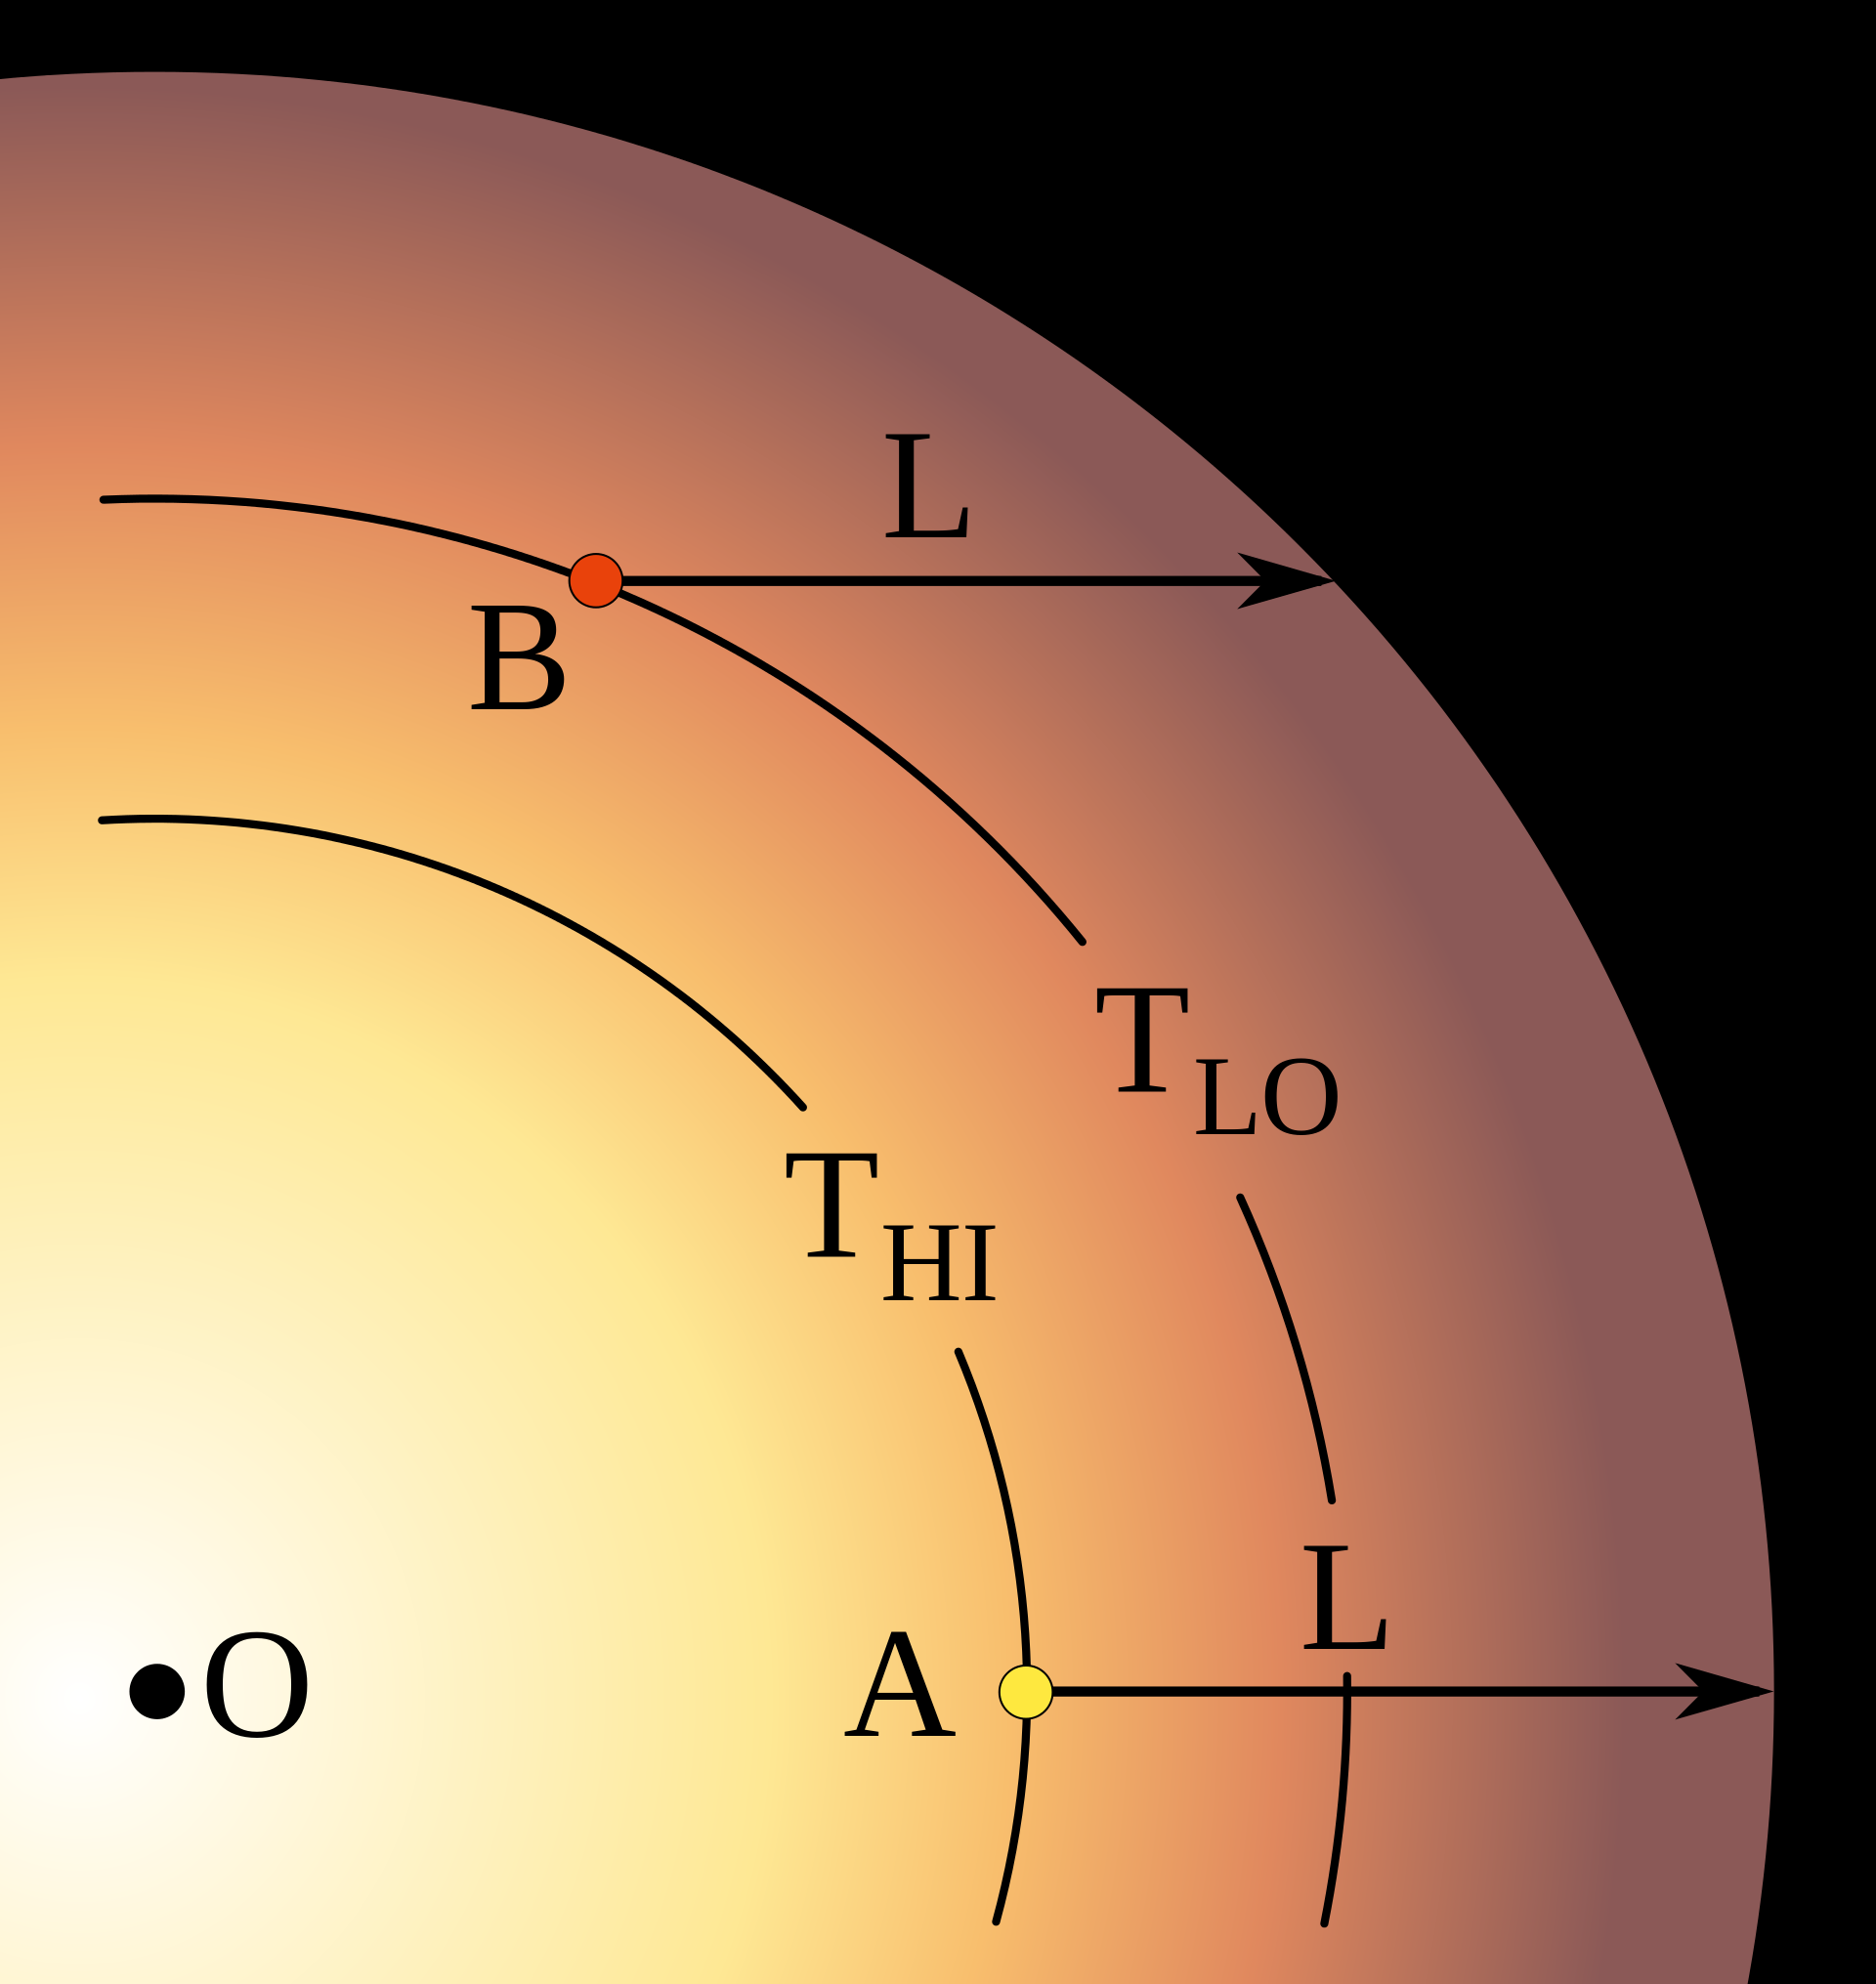
\includegraphics[scale=0.08]{Figures/limb_darkening.png}
    \caption{Εμηνεία του φαινομένου της αμαύρωσης του χείλους του 'Ηλιου σε οπτικά μήκη κύματος. Το εξωτερικό όριο αντιστοιχεί σε ακτίνα στην οποία τα φωτόνια που εκπέμπει ο αστέρας δεν υπόκεινται σε απορρόφηση. Ο παρατηρητής βλέπει στρώματα του Ήλιου που αντιστοιχούν σε οπτικό βάθος $\tau \approx 1$ (απόσταση L). Όταν παρατηρεί προς το κέντρο του Ηλιακού δίσκου, βλέπει βαθύτερα και θερμότερα, και άρα λαμπρότερα στρώματα, απ' ότι όταν παρατηρεί προς το χείλος του Ηλιακού δίσκου.}
    \label{fig:limb_darkening}
\end{figure}

Κάνοντας αναλύτικά τους υπολογισμούς, βρίσκουμε ότι ο μεγαλύτερος αριθμός φωτονίων με $\lambda = 5000 \ \text{\AA}$ προέρχονται από τον φλοιό που ορίζεται από την επιφάνεια για την οποία το οπτικό βάθος είναι $\tau = 4.5$ και την επιφάνεια για την οποία το οπτικό βάθος είναι $\tau = 0.7$. Επιφάνειες που βρίσκονται σε ακόμα μικρότερο βάθος από την επιφάνεια με $\tau = 0.7$, ουσιαστικά δεν παράγουν αρκετά οπτικά φωτόνια για να τις συμπεριλάβουμε και απλά θεωρούμε ότι τα φωτόνια που παράγονται στα κατώτερα στρώματα απλά διέρχονται από αυτές. Τον φλοιό αυτό τον ονομάζουμε \textbf{φωτόσφαιρα}.

Το ερώτημα τώρα είναι πόσο είναι το πάχος αυτού του σφαιρικού φλοιού που ορίζει τη φωτόσφαιρα του Ήλιου.
Θεωρώντας τα $\kappa_{\nu=5000 \ \text{\AA}} \equiv \kappa, \rho$ σταθερά σε αυτό το πάχος του φλοιού, τότε
$$\Delta S = S_{4.5} - S_{0.7} = \left. \frac{\tau}{\kappa \rho} \right|_{4.5} - \left. \frac{\tau}{\kappa \rho} \right|_{0.7} = \frac{4.5 - 0.7}{\kappa \rho} $$
Αντικαθιστώντας τις τιμές $\kappa = 0.03 \ \text{m$^2 $kg$^{-1}$}$ και $\rho = 2.1 \times 10^{-4} \ \text{kg m$^{-3}$}$ για την αδιαφάνεια και την μέση πυκνότητα του Ήλιου, τις οποίες γνωρίζουμε από παρατηρήσεις, προκύπτει ότι το πάχος του φλοιού από τον οποίο προέρχονται η πλειοψηφία των οπτικών φωτονίων είναι $$\Delta S \simeq 600 \ \text{km}$$
Λόγω του πολύ μικρού πάχους του φλοιού αυτού, το οποίο αντιστοιχεί στο $0.1 \%$ της ηλιακής ακτίνας, η φωτόσφαιρα πολλές φορές θεωρείται ως η επιφάνεια του Ήλιου. Όι επιφάνειες (και όλες οι ενδιάμεσες) που ορίζουν την φωτόσφαιρα του Ήλιου, χαρακτηρίζονται όπως είπαμε από διαφορετικές θερμοκρασίες καθώς αντιστοιχούν σε διαφορετικά βάθη. Γίνεται αντιληπτό πως η ενεργός θερμοκρασία του Ήλιου δεν χαρακτηρίζει κάποιο συγκεκριμένο στρώμα της φωτόσφαιρας, αλλά αποτελεί έναν εύχρηστο μέσο όρο.

Το εξαιρετικά μικρό πάχος της φωτόσφαιρας απαντάει στο ερώτημα του γιατί ο Ήλιος έχει σαφώς καθορισμένο περίγραμμα καθώς τα τηλεσκόπια δεν έχουν την απαραίτητα διακριτική ικανότητα να ξεχωρίσουν τον μικρό αυτό φλοιό σε σχέση με την ακτίνα του Ήλιου. Αν μπορούσαμε να διακρίνουμε αποστάσεις 600 χιλιομέτρων στον Ήλιο, τότε σαφώς το περίγραμμά του δεν θα ήταν τόσο καθαρό.




\subsection{Σύνοψη}
Η φασματική κατανομή μέλανος σώματος θερμοκρασίας $T_{\text{eff}}$ δίνεται από τον νόμο του Planck και σε καλή προσέγγιση συμφωνεί με την παρατηρούμενη φασματική κατανομή της ηλιακής ακτινοβολίας για  $T_{\text{eff}} = 5800 \ \text{K}$. Παρόλα αυτά, δεν συμπίπτουν τέλεια με τις διαφορές να οφείλονται στους εξής λόγους:
\begin{enumerate}
    \item Η ακτινοβολία του Ήλιου που φτάνει σε εμάς προέρχεται από διαφορετικά βάθη των εξωτερικών στρωμάτων του Ήλιου, τα οποία έχουν διαφορετικές θερμοκρασίες. Έτσι, η φωτεινή ένταση σε μια φασματική περιοχή είναι το άθροισμα των εντάσεων κατανομών που αντιστοιχούν σε διαφορετικές θερμοκρασίες.
    \item Στα μεγάλα (ραδιοφωνικά) και μικρά μήκη κύματος (υπεριώδες, ακτίνες-Χ κτλ) η ακτινοβολία του Ήλιου δεν είναι θερμικής φύσης, οπότε η έντασή της δεν έχει κανένα λόγο να ακολουθεί τον νόμο του Planck.
    \item Το ηλιακό φάσμα παρουσιάζει γραμμές απορρόφησης (γνωστές και ως γραμμές Fraunhofer) οι οποίες ελαττώνουν τη μέση ένταση της ακτινοβολίας σητν περιοχή που εμφανίζονται. Το φαινόμενο αυτό είναι ιδιαίτερα εμφανές στην περιοχή του ορίου συσσώρευσης των γραμμών της σειράς Balmer, που ονομάζεται ασυνέχεια Balmer.
    \item Τέλος, η ύλη που ακτινοβολεί θερμικά δεν βρίσκεται σε τοπική θερμοδυναμική ισορροπία, και άρα δεν ισχύει ακριβώς ο νόμος του Planck. Αξίζει να σημειωθεί όμως ότι η απόκλιση της κατανομής της έντασης της ηλιακής ακτινοβολίας από αυτή του μελανού σώματος, λόγω της μη ακριβούς θερμοδυναμικής ισορροπίας, είναι ασήμαντη σε σχέση με τις τρεις προηγούμενες αιτίες.
\end{enumerate}











